\documentclass[twoside]{book}

% Packages required by doxygen
\usepackage{fixltx2e}
\usepackage{calc}
\usepackage{doxygen}
\usepackage[export]{adjustbox} % also loads graphicx
\usepackage{graphicx}
\usepackage[utf8]{inputenc}
\usepackage{makeidx}
\usepackage{multicol}
\usepackage{multirow}
\PassOptionsToPackage{warn}{textcomp}
\usepackage{textcomp}
\usepackage[nointegrals]{wasysym}
\usepackage[table]{xcolor}

% Font selection
\usepackage[T1]{fontenc}
\usepackage[scaled=.90]{helvet}
\usepackage{courier}
\usepackage{amssymb}
\usepackage{sectsty}
\renewcommand{\familydefault}{\sfdefault}
\allsectionsfont{%
  \fontseries{bc}\selectfont%
  \color{darkgray}%
}
\renewcommand{\DoxyLabelFont}{%
  \fontseries{bc}\selectfont%
  \color{darkgray}%
}
\newcommand{\+}{\discretionary{\mbox{\scriptsize$\hookleftarrow$}}{}{}}

% Page & text layout
\usepackage{geometry}
\geometry{%
  a4paper,%
  top=2.5cm,%
  bottom=2.5cm,%
  left=2.5cm,%
  right=2.5cm%
}
\tolerance=750
\hfuzz=15pt
\hbadness=750
\setlength{\emergencystretch}{15pt}
\setlength{\parindent}{0cm}
\setlength{\parskip}{3ex plus 2ex minus 2ex}
\makeatletter
\renewcommand{\paragraph}{%
  \@startsection{paragraph}{4}{0ex}{-1.0ex}{1.0ex}{%
    \normalfont\normalsize\bfseries\SS@parafont%
  }%
}
\renewcommand{\subparagraph}{%
  \@startsection{subparagraph}{5}{0ex}{-1.0ex}{1.0ex}{%
    \normalfont\normalsize\bfseries\SS@subparafont%
  }%
}
\makeatother

% Headers & footers
\usepackage{fancyhdr}
\pagestyle{fancyplain}
\fancyhead[LE]{\fancyplain{}{\bfseries\thepage}}
\fancyhead[CE]{\fancyplain{}{}}
\fancyhead[RE]{\fancyplain{}{\bfseries\leftmark}}
\fancyhead[LO]{\fancyplain{}{\bfseries\rightmark}}
\fancyhead[CO]{\fancyplain{}{}}
\fancyhead[RO]{\fancyplain{}{\bfseries\thepage}}
\fancyfoot[LE]{\fancyplain{}{}}
\fancyfoot[CE]{\fancyplain{}{}}
\fancyfoot[RE]{\fancyplain{}{\bfseries\scriptsize Generated by Doxygen }}
\fancyfoot[LO]{\fancyplain{}{\bfseries\scriptsize Generated by Doxygen }}
\fancyfoot[CO]{\fancyplain{}{}}
\fancyfoot[RO]{\fancyplain{}{}}
\renewcommand{\footrulewidth}{0.4pt}
\renewcommand{\chaptermark}[1]{%
  \markboth{#1}{}%
}
\renewcommand{\sectionmark}[1]{%
  \markright{\thesection\ #1}%
}

% Indices & bibliography
\usepackage{natbib}
\usepackage[titles]{tocloft}
\setcounter{tocdepth}{3}
\setcounter{secnumdepth}{5}
\makeindex

% Hyperlinks (required, but should be loaded last)
\usepackage{ifpdf}
\ifpdf
  \usepackage[pdftex,pagebackref=true]{hyperref}
\else
  \usepackage[ps2pdf,pagebackref=true]{hyperref}
\fi
\hypersetup{%
  colorlinks=true,%
  linkcolor=blue,%
  citecolor=blue,%
  unicode%
}

% Custom commands
\newcommand{\clearemptydoublepage}{%
  \newpage{\pagestyle{empty}\cleardoublepage}%
}

\usepackage{caption}
\captionsetup{labelsep=space,justification=centering,font={bf},singlelinecheck=off,skip=4pt,position=top}

%===== C O N T E N T S =====

\begin{document}

% Titlepage & ToC
\hypersetup{pageanchor=false,
             bookmarksnumbered=true,
             pdfencoding=unicode
            }
\pagenumbering{alph}
\begin{titlepage}
\vspace*{7cm}
\begin{center}%
{\Large Scheduler Strong A\+PA \\[1ex]\large Pre-\/\+Release }\\
\vspace*{1cm}
{\large Generated by Doxygen 1.8.13}\\
\end{center}
\end{titlepage}
\clearemptydoublepage
\pagenumbering{roman}
\tableofcontents
\clearemptydoublepage
\pagenumbering{arabic}
\hypersetup{pageanchor=true}

%--- Begin generated contents ---
\chapter{Documentation for Strong A\+PA Scheduler to be added to R\+T\+E\+MS}
\label{index}\hypertarget{index}{}\hypertarget{index_Introduction}{}\section{Introduction}\label{index_Introduction}
This project aims to add the Arbitrary Processor Affinity (A\+PA) scheduler to R\+T\+E\+MS. A\+PA scheduler would allow higher-\/priority tasks to be ”dislodged” or moved among processors in order to make space for lower priority tasks that are limited by affinity constraints.

We model the task to processor mapping as a bi-\/partite graph. An edge denotes a task being assigned a C\+PU.

When a processor A gets free, it looks for all the possible tasks that it can run. This includes the ready waiting task which have the processor A in their affinity set as well as the ready waiting task which has a processor B in its affinity set, but the processor B is executing a task which can be shifted to prcessor A and therefore the ready-\/waiting task being executed.

This algorithm runs recursively to find any possible task to processor mapping that does not violate the priority ordering and generates a mapping with the highest total priority of tasks begin executed.

Learn more about the project from the link \+: \href{https://summerofcode.withgoogle.com/projects/#5074448194994176}{\tt https\+://summerofcode.\+withgoogle.\+com/projects/\#5074448194994176} 
\chapter{Module Index}
\section{Modules}
Here is a list of all modules\+:\begin{DoxyCompactList}
\item \contentsline{section}{Strong A\+PA Scheduler}{\pageref{group__RTEMSScoreSchedulerStrongAPA}}{}
\end{DoxyCompactList}

\chapter{Class Index}
\section{Class List}
Here are the classes, structs, unions and interfaces with brief descriptions\+:\begin{DoxyCompactList}
\item\contentsline{section}{\hyperlink{structScheduler__strong__APA__Context}{Scheduler\+\_\+strong\+\_\+\+A\+P\+A\+\_\+\+Context} \\*Scheduler context for Strong A\+PA scheduler }{\pageref{structScheduler__strong__APA__Context}}{}
\item\contentsline{section}{\hyperlink{structScheduler__strong__APA__CPU}{Scheduler\+\_\+strong\+\_\+\+A\+P\+A\+\_\+\+C\+PU} }{\pageref{structScheduler__strong__APA__CPU}}{}
\item\contentsline{section}{\hyperlink{structScheduler__strong__APA__Node}{Scheduler\+\_\+strong\+\_\+\+A\+P\+A\+\_\+\+Node} \\*Scheduler node specialization for Strong A\+PA schedulers }{\pageref{structScheduler__strong__APA__Node}}{}
\end{DoxyCompactList}

\chapter{File Index}
\section{File List}
Here is a list of all files with brief descriptions\+:\begin{DoxyCompactList}
\item\contentsline{section}{\hyperlink{schedulerstrongapa_8c}{schedulerstrongapa.\+c} }{\pageref{schedulerstrongapa_8c}}{}
\item\contentsline{section}{\hyperlink{schedulerstrongapa_8h}{schedulerstrongapa.\+h} \\*Strong A\+PA Scheduler A\+PI }{\pageref{schedulerstrongapa_8h}}{}
\end{DoxyCompactList}

\chapter{Module Documentation}
\hypertarget{group__RTEMSScoreSchedulerStrongAPA}{}\section{Strong A\+PA Scheduler}
\label{group__RTEMSScoreSchedulerStrongAPA}\index{Strong A\+P\+A Scheduler@{Strong A\+P\+A Scheduler}}


Strong A\+PA Scheduler.  


\subsection*{Files}
\begin{DoxyCompactItemize}
\item 
file \hyperlink{schedulerstrongapa_8c}{schedulerstrongapa.\+c}
\begin{DoxyCompactList}\small\item\em Strong A\+PA Scheduler Implementation. \end{DoxyCompactList}\item 
file \hyperlink{schedulerstrongapa_8h}{schedulerstrongapa.\+h}
\begin{DoxyCompactList}\small\item\em Strong A\+PA Scheduler A\+PI. \end{DoxyCompactList}\end{DoxyCompactItemize}
\subsection*{Classes}
\begin{DoxyCompactItemize}
\item 
struct \hyperlink{structScheduler__strong__APA__Node}{Scheduler\+\_\+strong\+\_\+\+A\+P\+A\+\_\+\+Node}
\begin{DoxyCompactList}\small\item\em Scheduler node specialization for Strong A\+PA schedulers. \end{DoxyCompactList}\item 
struct \hyperlink{structScheduler__strong__APA__CPU}{Scheduler\+\_\+strong\+\_\+\+A\+P\+A\+\_\+\+C\+PU}
\begin{DoxyCompactList}\small\item\em C\+PU related variables and a C\+P\+U\+\_\+\+Control to implement B\+FS. \end{DoxyCompactList}\item 
struct \hyperlink{structScheduler__strong__APA__Context}{Scheduler\+\_\+strong\+\_\+\+A\+P\+A\+\_\+\+Context}
\begin{DoxyCompactList}\small\item\em Scheduler context and node definition for Strong A\+PA scheduler. \end{DoxyCompactList}\end{DoxyCompactItemize}
\subsection*{Macros}
\begin{DoxyCompactItemize}
\item 
\#define \hyperlink{group__RTEMSScoreSchedulerStrongAPA_gab917bac4c45882604043daa2f4fafcfb}{S\+C\+H\+E\+D\+U\+L\+E\+R\+\_\+\+S\+T\+R\+O\+N\+G\+\_\+\+A\+P\+A\+\_\+\+M\+A\+X\+I\+M\+U\+M\+\_\+\+P\+R\+I\+O\+R\+I\+TY}~255
\item 
\#define \hyperlink{group__RTEMSScoreSchedulerStrongAPA_ga98b37281082c0be47dc489eed554c5cc}{S\+C\+H\+E\+D\+U\+L\+E\+R\+\_\+\+S\+T\+R\+O\+N\+G\+\_\+\+A\+P\+A\+\_\+\+E\+N\+T\+R\+Y\+\_\+\+P\+O\+I\+N\+TS}
\begin{DoxyCompactList}\small\item\em Entry points for the Strong A\+PA Scheduler. \end{DoxyCompactList}\end{DoxyCompactItemize}
\subsection*{Functions}
\begin{DoxyCompactItemize}
\item 
void \hyperlink{group__RTEMSScoreSchedulerStrongAPA_gafcd6fde337d7542784698219322b6365}{\+\_\+\+Scheduler\+\_\+strong\+\_\+\+A\+P\+A\+\_\+\+Initialize} (const Scheduler\+\_\+\+Control $\ast$scheduler)
\begin{DoxyCompactList}\small\item\em Initializes the scheduler. \end{DoxyCompactList}\item 
void \hyperlink{group__RTEMSScoreSchedulerStrongAPA_ga1cde4345d4dc0b5a37a696fa446bb47e}{\+\_\+\+Scheduler\+\_\+strong\+\_\+\+A\+P\+A\+\_\+\+Node\+\_\+initialize} (const Scheduler\+\_\+\+Control $\ast$scheduler, Scheduler\+\_\+\+Node $\ast$node, Thread\+\_\+\+Control $\ast$the\+\_\+thread, Priority\+\_\+\+Control priority)
\begin{DoxyCompactList}\small\item\em Initializes the node with the given priority. \end{DoxyCompactList}\item 
void \hyperlink{group__RTEMSScoreSchedulerStrongAPA_ga0f3ca9f9dcaff88a5df871622caf5e3f}{\+\_\+\+Scheduler\+\_\+strong\+\_\+\+A\+P\+A\+\_\+\+Block} (const Scheduler\+\_\+\+Control $\ast$scheduler, Thread\+\_\+\+Control $\ast$the\+\_\+thread, Scheduler\+\_\+\+Node $\ast$node)
\begin{DoxyCompactList}\small\item\em Blocks the thread. \end{DoxyCompactList}\item 
void \hyperlink{group__RTEMSScoreSchedulerStrongAPA_ga6b96ab0939d82ee5813092159265840e}{\+\_\+\+Scheduler\+\_\+strong\+\_\+\+A\+P\+A\+\_\+\+Unblock} (const Scheduler\+\_\+\+Control $\ast$scheduler, Thread\+\_\+\+Control $\ast$the\+\_\+thread, Scheduler\+\_\+\+Node $\ast$node)
\begin{DoxyCompactList}\small\item\em Unblocks the thread. \end{DoxyCompactList}\item 
void \hyperlink{group__RTEMSScoreSchedulerStrongAPA_ga3cdc0079d2d16a392834bd03b5115ad9}{\+\_\+\+Scheduler\+\_\+strong\+\_\+\+A\+P\+A\+\_\+\+Update\+\_\+priority} (const Scheduler\+\_\+\+Control $\ast$scheduler, Thread\+\_\+\+Control $\ast$the\+\_\+thread, Scheduler\+\_\+\+Node $\ast$node)
\begin{DoxyCompactList}\small\item\em Updates the priority of the node. \end{DoxyCompactList}\item 
bool \hyperlink{group__RTEMSScoreSchedulerStrongAPA_gad863eddc3fa4e2d785fb64af6505e90b}{\+\_\+\+Scheduler\+\_\+strong\+\_\+\+A\+P\+A\+\_\+\+Ask\+\_\+for\+\_\+help} (const Scheduler\+\_\+\+Control $\ast$scheduler, Thread\+\_\+\+Control $\ast$the\+\_\+thread, Scheduler\+\_\+\+Node $\ast$node)
\begin{DoxyCompactList}\small\item\em Asks for help. \end{DoxyCompactList}\item 
void \hyperlink{group__RTEMSScoreSchedulerStrongAPA_ga7809e64065ec5d291f3dc82220a68d3f}{\+\_\+\+Scheduler\+\_\+strong\+\_\+\+A\+P\+A\+\_\+\+Reconsider\+\_\+help\+\_\+request} (const Scheduler\+\_\+\+Control $\ast$scheduler, Thread\+\_\+\+Control $\ast$the\+\_\+thread, Scheduler\+\_\+\+Node $\ast$node)
\begin{DoxyCompactList}\small\item\em Reconsiders help request. \end{DoxyCompactList}\item 
void \hyperlink{group__RTEMSScoreSchedulerStrongAPA_gaf43eb65a6fbbe2826ca4cec68a930cb5}{\+\_\+\+Scheduler\+\_\+strong\+\_\+\+A\+P\+A\+\_\+\+Withdraw\+\_\+node} (const Scheduler\+\_\+\+Control $\ast$scheduler, Thread\+\_\+\+Control $\ast$the\+\_\+thread, Scheduler\+\_\+\+Node $\ast$node, Thread\+\_\+\+Scheduler\+\_\+state next\+\_\+state)
\begin{DoxyCompactList}\small\item\em Withdraws the node. \end{DoxyCompactList}\item 
void \hyperlink{group__RTEMSScoreSchedulerStrongAPA_ga6ac09dac24785561fd7c5ee5bbd8f5ca}{\+\_\+\+Scheduler\+\_\+strong\+\_\+\+A\+P\+A\+\_\+\+Add\+\_\+processor} (const Scheduler\+\_\+\+Control $\ast$scheduler, Thread\+\_\+\+Control $\ast$idle)
\begin{DoxyCompactList}\small\item\em Adds the idle thread to a processor. \end{DoxyCompactList}\item 
Thread\+\_\+\+Control $\ast$ \hyperlink{group__RTEMSScoreSchedulerStrongAPA_gac83f4ab63b404cdfea31e572fa9590a5}{\+\_\+\+Scheduler\+\_\+strong\+\_\+\+A\+P\+A\+\_\+\+Remove\+\_\+processor} (const Scheduler\+\_\+\+Control $\ast$scheduler, struct Per\+\_\+\+C\+P\+U\+\_\+\+Control $\ast$cpu)
\begin{DoxyCompactList}\small\item\em Removes an idle thread from the given cpu. \end{DoxyCompactList}\item 
void \hyperlink{group__RTEMSScoreSchedulerStrongAPA_ga0720c2d79f2b6dd8e91d19879f72b8c7}{\+\_\+\+Scheduler\+\_\+strong\+\_\+\+A\+P\+A\+\_\+\+Yield} (const Scheduler\+\_\+\+Control $\ast$scheduler, Thread\+\_\+\+Control $\ast$the\+\_\+thread, Scheduler\+\_\+\+Node $\ast$node)
\begin{DoxyCompactList}\small\item\em Performs a yield operation. \end{DoxyCompactList}\item 
void \hyperlink{group__RTEMSScoreSchedulerStrongAPA_gaaf3d646f61984f8a69ff1850a020fa1b}{\+\_\+\+Scheduler\+\_\+strong\+\_\+\+A\+P\+A\+\_\+\+Start\+\_\+idle} (const Scheduler\+\_\+\+Control $\ast$scheduler, Thread\+\_\+\+Control $\ast$idle, struct Per\+\_\+\+C\+P\+U\+\_\+\+Control $\ast$cpu)
\begin{DoxyCompactList}\small\item\em Starts an idle thread. \end{DoxyCompactList}\item 
bool \hyperlink{group__RTEMSScoreSchedulerStrongAPA_ga63ef624a9881cf77a2b1eef2c6f05223}{\+\_\+\+Scheduler\+\_\+strong\+\_\+\+A\+P\+A\+\_\+\+Set\+\_\+affinity} (const Scheduler\+\_\+\+Control $\ast$scheduler, Thread\+\_\+\+Control $\ast$thread, Scheduler\+\_\+\+Node $\ast$node\+\_\+base, const Processor\+\_\+mask $\ast$affinity)
\begin{DoxyCompactList}\small\item\em Sets the affinity . \end{DoxyCompactList}\end{DoxyCompactItemize}


\subsection{Detailed Description}
Strong A\+PA Scheduler. 

This is an implementation of the Strong A\+PA scheduler defined by Cerqueira et al. in Linux\textquotesingle{}s Processor Affinity A\+PI, Refined\+: Shifting Real-\/\+Time Tasks Towards Higher Schedulability.

The scheduled and ready nodes are accessed via the \hyperlink{structScheduler__strong__APA__Context_a0c445c35a07b8aa14f9d76c6dfb4916c}{Scheduler\+\_\+strong\+\_\+\+A\+P\+A\+\_\+\+Context\+::\+Ready} which helps in backtracking when a node which is executing on a C\+PU gets blocked. New node is allocated to the cpu by checking all the executing nodes in the affinity set of the node and the subsequent nodes executing on the processors in its affinity set. 

\subsection{Macro Definition Documentation}
\mbox{\Hypertarget{group__RTEMSScoreSchedulerStrongAPA_ga98b37281082c0be47dc489eed554c5cc}\label{group__RTEMSScoreSchedulerStrongAPA_ga98b37281082c0be47dc489eed554c5cc}} 
\index{Strong A\+P\+A Scheduler@{Strong A\+P\+A Scheduler}!S\+C\+H\+E\+D\+U\+L\+E\+R\+\_\+\+S\+T\+R\+O\+N\+G\+\_\+\+A\+P\+A\+\_\+\+E\+N\+T\+R\+Y\+\_\+\+P\+O\+I\+N\+TS@{S\+C\+H\+E\+D\+U\+L\+E\+R\+\_\+\+S\+T\+R\+O\+N\+G\+\_\+\+A\+P\+A\+\_\+\+E\+N\+T\+R\+Y\+\_\+\+P\+O\+I\+N\+TS}}
\index{S\+C\+H\+E\+D\+U\+L\+E\+R\+\_\+\+S\+T\+R\+O\+N\+G\+\_\+\+A\+P\+A\+\_\+\+E\+N\+T\+R\+Y\+\_\+\+P\+O\+I\+N\+TS@{S\+C\+H\+E\+D\+U\+L\+E\+R\+\_\+\+S\+T\+R\+O\+N\+G\+\_\+\+A\+P\+A\+\_\+\+E\+N\+T\+R\+Y\+\_\+\+P\+O\+I\+N\+TS}!Strong A\+P\+A Scheduler@{Strong A\+P\+A Scheduler}}
\subsubsection{\texorpdfstring{S\+C\+H\+E\+D\+U\+L\+E\+R\+\_\+\+S\+T\+R\+O\+N\+G\+\_\+\+A\+P\+A\+\_\+\+E\+N\+T\+R\+Y\+\_\+\+P\+O\+I\+N\+TS}{SCHEDULER\_STRONG\_APA\_ENTRY\_POINTS}}
{\footnotesize\ttfamily \#define S\+C\+H\+E\+D\+U\+L\+E\+R\+\_\+\+S\+T\+R\+O\+N\+G\+\_\+\+A\+P\+A\+\_\+\+E\+N\+T\+R\+Y\+\_\+\+P\+O\+I\+N\+TS}

{\bfseries Value\+:}
\begin{DoxyCode}
\{ \(\backslash\)
    \_Scheduler\_strong\_APA\_Initialize, \(\backslash\)
    \_Scheduler\_default\_Schedule, \(\backslash\)
    \_Scheduler\_strong\_APA\_Yield, \(\backslash\)
    \_Scheduler\_strong\_APA\_Block, \(\backslash\)
    \_Scheduler\_strong\_APA\_Unblock, \(\backslash\)
    \_Scheduler\_strong\_APA\_Update\_priority, \(\backslash\)
    \_Scheduler\_default\_Map\_priority, \(\backslash\)
    \_Scheduler\_default\_Unmap\_priority, \(\backslash\)
    \_Scheduler\_strong\_APA\_Ask\_for\_help, \(\backslash\)
    \_Scheduler\_strong\_APA\_Reconsider\_help\_request, \(\backslash\)
    \_Scheduler\_strong\_APA\_Withdraw\_node, \(\backslash\)
    \_Scheduler\_default\_Pin\_or\_unpin, \(\backslash\)
    \_Scheduler\_default\_Pin\_or\_unpin, \(\backslash\)
    \_Scheduler\_strong\_APA\_Add\_processor, \(\backslash\)
    \_Scheduler\_strong\_APA\_Remove\_processor, \(\backslash\)
    \_Scheduler\_strong\_APA\_Node\_initialize, \(\backslash\)
    \_Scheduler\_default\_Node\_destroy, \(\backslash\)
    \_Scheduler\_default\_Release\_job, \(\backslash\)
    \_Scheduler\_default\_Cancel\_job, \(\backslash\)
    \_Scheduler\_default\_Tick, \(\backslash\)
    \_Scheduler\_strong\_APA\_Start\_idle, \(\backslash\)
    \_Scheduler\_strong\_APA\_Set\_affinity \(\backslash\)
  \}
\end{DoxyCode}


Entry points for the Strong A\+PA Scheduler. 



Definition at line 151 of file schedulerstrongapa.\+h.

\mbox{\Hypertarget{group__RTEMSScoreSchedulerStrongAPA_gab917bac4c45882604043daa2f4fafcfb}\label{group__RTEMSScoreSchedulerStrongAPA_gab917bac4c45882604043daa2f4fafcfb}} 
\index{Strong A\+P\+A Scheduler@{Strong A\+P\+A Scheduler}!S\+C\+H\+E\+D\+U\+L\+E\+R\+\_\+\+S\+T\+R\+O\+N\+G\+\_\+\+A\+P\+A\+\_\+\+M\+A\+X\+I\+M\+U\+M\+\_\+\+P\+R\+I\+O\+R\+I\+TY@{S\+C\+H\+E\+D\+U\+L\+E\+R\+\_\+\+S\+T\+R\+O\+N\+G\+\_\+\+A\+P\+A\+\_\+\+M\+A\+X\+I\+M\+U\+M\+\_\+\+P\+R\+I\+O\+R\+I\+TY}}
\index{S\+C\+H\+E\+D\+U\+L\+E\+R\+\_\+\+S\+T\+R\+O\+N\+G\+\_\+\+A\+P\+A\+\_\+\+M\+A\+X\+I\+M\+U\+M\+\_\+\+P\+R\+I\+O\+R\+I\+TY@{S\+C\+H\+E\+D\+U\+L\+E\+R\+\_\+\+S\+T\+R\+O\+N\+G\+\_\+\+A\+P\+A\+\_\+\+M\+A\+X\+I\+M\+U\+M\+\_\+\+P\+R\+I\+O\+R\+I\+TY}!Strong A\+P\+A Scheduler@{Strong A\+P\+A Scheduler}}
\subsubsection{\texorpdfstring{S\+C\+H\+E\+D\+U\+L\+E\+R\+\_\+\+S\+T\+R\+O\+N\+G\+\_\+\+A\+P\+A\+\_\+\+M\+A\+X\+I\+M\+U\+M\+\_\+\+P\+R\+I\+O\+R\+I\+TY}{SCHEDULER\_STRONG\_APA\_MAXIMUM\_PRIORITY}}
{\footnotesize\ttfamily \#define S\+C\+H\+E\+D\+U\+L\+E\+R\+\_\+\+S\+T\+R\+O\+N\+G\+\_\+\+A\+P\+A\+\_\+\+M\+A\+X\+I\+M\+U\+M\+\_\+\+P\+R\+I\+O\+R\+I\+TY~255}



Definition at line 146 of file schedulerstrongapa.\+h.



\subsection{Function Documentation}
\mbox{\Hypertarget{group__RTEMSScoreSchedulerStrongAPA_ga6ac09dac24785561fd7c5ee5bbd8f5ca}\label{group__RTEMSScoreSchedulerStrongAPA_ga6ac09dac24785561fd7c5ee5bbd8f5ca}} 
\index{Strong A\+P\+A Scheduler@{Strong A\+P\+A Scheduler}!\+\_\+\+Scheduler\+\_\+strong\+\_\+\+A\+P\+A\+\_\+\+Add\+\_\+processor@{\+\_\+\+Scheduler\+\_\+strong\+\_\+\+A\+P\+A\+\_\+\+Add\+\_\+processor}}
\index{\+\_\+\+Scheduler\+\_\+strong\+\_\+\+A\+P\+A\+\_\+\+Add\+\_\+processor@{\+\_\+\+Scheduler\+\_\+strong\+\_\+\+A\+P\+A\+\_\+\+Add\+\_\+processor}!Strong A\+P\+A Scheduler@{Strong A\+P\+A Scheduler}}
\subsubsection{\texorpdfstring{\+\_\+\+Scheduler\+\_\+strong\+\_\+\+A\+P\+A\+\_\+\+Add\+\_\+processor()}{\_Scheduler\_strong\_APA\_Add\_processor()}}
{\footnotesize\ttfamily void \+\_\+\+Scheduler\+\_\+strong\+\_\+\+A\+P\+A\+\_\+\+Add\+\_\+processor (\begin{DoxyParamCaption}\item[{const Scheduler\+\_\+\+Control $\ast$}]{scheduler,  }\item[{Thread\+\_\+\+Control $\ast$}]{idle }\end{DoxyParamCaption})}



Adds the idle thread to a processor. 


\begin{DoxyParams}[1]{Parameters}
 & {\em scheduler} & The scheduler control instance. \\
\hline
\mbox{\tt in,out}  & {\em The} & idle thread to add to the processor. \\
\hline
\end{DoxyParams}


Definition at line 886 of file schedulerstrongapa.\+c.

\mbox{\Hypertarget{group__RTEMSScoreSchedulerStrongAPA_gad863eddc3fa4e2d785fb64af6505e90b}\label{group__RTEMSScoreSchedulerStrongAPA_gad863eddc3fa4e2d785fb64af6505e90b}} 
\index{Strong A\+P\+A Scheduler@{Strong A\+P\+A Scheduler}!\+\_\+\+Scheduler\+\_\+strong\+\_\+\+A\+P\+A\+\_\+\+Ask\+\_\+for\+\_\+help@{\+\_\+\+Scheduler\+\_\+strong\+\_\+\+A\+P\+A\+\_\+\+Ask\+\_\+for\+\_\+help}}
\index{\+\_\+\+Scheduler\+\_\+strong\+\_\+\+A\+P\+A\+\_\+\+Ask\+\_\+for\+\_\+help@{\+\_\+\+Scheduler\+\_\+strong\+\_\+\+A\+P\+A\+\_\+\+Ask\+\_\+for\+\_\+help}!Strong A\+P\+A Scheduler@{Strong A\+P\+A Scheduler}}
\subsubsection{\texorpdfstring{\+\_\+\+Scheduler\+\_\+strong\+\_\+\+A\+P\+A\+\_\+\+Ask\+\_\+for\+\_\+help()}{\_Scheduler\_strong\_APA\_Ask\_for\_help()}}
{\footnotesize\ttfamily bool \+\_\+\+Scheduler\+\_\+strong\+\_\+\+A\+P\+A\+\_\+\+Ask\+\_\+for\+\_\+help (\begin{DoxyParamCaption}\item[{const Scheduler\+\_\+\+Control $\ast$}]{scheduler,  }\item[{Thread\+\_\+\+Control $\ast$}]{the\+\_\+thread,  }\item[{Scheduler\+\_\+\+Node $\ast$}]{node }\end{DoxyParamCaption})}



Asks for help. 


\begin{DoxyParams}{Parameters}
{\em scheduler} & The scheduler control instance. \\
\hline
{\em the\+\_\+thread} & The thread that asks for help. \\
\hline
{\em node} & The node of {\itshape the\+\_\+thread}.\\
\hline
\end{DoxyParams}

\begin{DoxyRetVals}{Return values}
{\em true} & The request for help was successful. \\
\hline
{\em false} & The request for help was not successful. \\
\hline
\end{DoxyRetVals}


Definition at line 822 of file schedulerstrongapa.\+c.

\mbox{\Hypertarget{group__RTEMSScoreSchedulerStrongAPA_ga0f3ca9f9dcaff88a5df871622caf5e3f}\label{group__RTEMSScoreSchedulerStrongAPA_ga0f3ca9f9dcaff88a5df871622caf5e3f}} 
\index{Strong A\+P\+A Scheduler@{Strong A\+P\+A Scheduler}!\+\_\+\+Scheduler\+\_\+strong\+\_\+\+A\+P\+A\+\_\+\+Block@{\+\_\+\+Scheduler\+\_\+strong\+\_\+\+A\+P\+A\+\_\+\+Block}}
\index{\+\_\+\+Scheduler\+\_\+strong\+\_\+\+A\+P\+A\+\_\+\+Block@{\+\_\+\+Scheduler\+\_\+strong\+\_\+\+A\+P\+A\+\_\+\+Block}!Strong A\+P\+A Scheduler@{Strong A\+P\+A Scheduler}}
\subsubsection{\texorpdfstring{\+\_\+\+Scheduler\+\_\+strong\+\_\+\+A\+P\+A\+\_\+\+Block()}{\_Scheduler\_strong\_APA\_Block()}}
{\footnotesize\ttfamily void \+\_\+\+Scheduler\+\_\+strong\+\_\+\+A\+P\+A\+\_\+\+Block (\begin{DoxyParamCaption}\item[{const Scheduler\+\_\+\+Control $\ast$}]{scheduler,  }\item[{Thread\+\_\+\+Control $\ast$}]{the\+\_\+thread,  }\item[{Scheduler\+\_\+\+Node $\ast$}]{node }\end{DoxyParamCaption})}



Blocks the thread. 


\begin{DoxyParams}[1]{Parameters}
 & {\em scheduler} & The scheduler control instance. \\
\hline
\mbox{\tt in,out}  & {\em the\+\_\+thread} & The thread to block. \\
\hline
\mbox{\tt in,out}  & {\em node} & The node of the thread to block. \\
\hline
\end{DoxyParams}


Definition at line 759 of file schedulerstrongapa.\+c.

\mbox{\Hypertarget{group__RTEMSScoreSchedulerStrongAPA_gafcd6fde337d7542784698219322b6365}\label{group__RTEMSScoreSchedulerStrongAPA_gafcd6fde337d7542784698219322b6365}} 
\index{Strong A\+P\+A Scheduler@{Strong A\+P\+A Scheduler}!\+\_\+\+Scheduler\+\_\+strong\+\_\+\+A\+P\+A\+\_\+\+Initialize@{\+\_\+\+Scheduler\+\_\+strong\+\_\+\+A\+P\+A\+\_\+\+Initialize}}
\index{\+\_\+\+Scheduler\+\_\+strong\+\_\+\+A\+P\+A\+\_\+\+Initialize@{\+\_\+\+Scheduler\+\_\+strong\+\_\+\+A\+P\+A\+\_\+\+Initialize}!Strong A\+P\+A Scheduler@{Strong A\+P\+A Scheduler}}
\subsubsection{\texorpdfstring{\+\_\+\+Scheduler\+\_\+strong\+\_\+\+A\+P\+A\+\_\+\+Initialize()}{\_Scheduler\_strong\_APA\_Initialize()}}
{\footnotesize\ttfamily void \+\_\+\+Scheduler\+\_\+strong\+\_\+\+A\+P\+A\+\_\+\+Initialize (\begin{DoxyParamCaption}\item[{const Scheduler\+\_\+\+Control $\ast$}]{scheduler }\end{DoxyParamCaption})}



Initializes the scheduler. 


\begin{DoxyParams}{Parameters}
{\em scheduler} & The scheduler to initialize. \\
\hline
\end{DoxyParams}


Definition at line 732 of file schedulerstrongapa.\+c.

\mbox{\Hypertarget{group__RTEMSScoreSchedulerStrongAPA_ga1cde4345d4dc0b5a37a696fa446bb47e}\label{group__RTEMSScoreSchedulerStrongAPA_ga1cde4345d4dc0b5a37a696fa446bb47e}} 
\index{Strong A\+P\+A Scheduler@{Strong A\+P\+A Scheduler}!\+\_\+\+Scheduler\+\_\+strong\+\_\+\+A\+P\+A\+\_\+\+Node\+\_\+initialize@{\+\_\+\+Scheduler\+\_\+strong\+\_\+\+A\+P\+A\+\_\+\+Node\+\_\+initialize}}
\index{\+\_\+\+Scheduler\+\_\+strong\+\_\+\+A\+P\+A\+\_\+\+Node\+\_\+initialize@{\+\_\+\+Scheduler\+\_\+strong\+\_\+\+A\+P\+A\+\_\+\+Node\+\_\+initialize}!Strong A\+P\+A Scheduler@{Strong A\+P\+A Scheduler}}
\subsubsection{\texorpdfstring{\+\_\+\+Scheduler\+\_\+strong\+\_\+\+A\+P\+A\+\_\+\+Node\+\_\+initialize()}{\_Scheduler\_strong\_APA\_Node\_initialize()}}
{\footnotesize\ttfamily void \+\_\+\+Scheduler\+\_\+strong\+\_\+\+A\+P\+A\+\_\+\+Node\+\_\+initialize (\begin{DoxyParamCaption}\item[{const Scheduler\+\_\+\+Control $\ast$}]{scheduler,  }\item[{Scheduler\+\_\+\+Node $\ast$}]{node,  }\item[{Thread\+\_\+\+Control $\ast$}]{the\+\_\+thread,  }\item[{Priority\+\_\+\+Control}]{priority }\end{DoxyParamCaption})}



Initializes the node with the given priority. 


\begin{DoxyParams}[1]{Parameters}
 & {\em scheduler} & The scheduler control instance. \\
\hline
\mbox{\tt out}  & {\em node} & The node to initialize. \\
\hline
 & {\em the\+\_\+thread} & The thread of the node to initialize. \\
\hline
 & {\em priority} & The priority for {\itshape node}. \\
\hline
\end{DoxyParams}


Definition at line 935 of file schedulerstrongapa.\+c.

\mbox{\Hypertarget{group__RTEMSScoreSchedulerStrongAPA_ga7809e64065ec5d291f3dc82220a68d3f}\label{group__RTEMSScoreSchedulerStrongAPA_ga7809e64065ec5d291f3dc82220a68d3f}} 
\index{Strong A\+P\+A Scheduler@{Strong A\+P\+A Scheduler}!\+\_\+\+Scheduler\+\_\+strong\+\_\+\+A\+P\+A\+\_\+\+Reconsider\+\_\+help\+\_\+request@{\+\_\+\+Scheduler\+\_\+strong\+\_\+\+A\+P\+A\+\_\+\+Reconsider\+\_\+help\+\_\+request}}
\index{\+\_\+\+Scheduler\+\_\+strong\+\_\+\+A\+P\+A\+\_\+\+Reconsider\+\_\+help\+\_\+request@{\+\_\+\+Scheduler\+\_\+strong\+\_\+\+A\+P\+A\+\_\+\+Reconsider\+\_\+help\+\_\+request}!Strong A\+P\+A Scheduler@{Strong A\+P\+A Scheduler}}
\subsubsection{\texorpdfstring{\+\_\+\+Scheduler\+\_\+strong\+\_\+\+A\+P\+A\+\_\+\+Reconsider\+\_\+help\+\_\+request()}{\_Scheduler\_strong\_APA\_Reconsider\_help\_request()}}
{\footnotesize\ttfamily void \+\_\+\+Scheduler\+\_\+strong\+\_\+\+A\+P\+A\+\_\+\+Reconsider\+\_\+help\+\_\+request (\begin{DoxyParamCaption}\item[{const Scheduler\+\_\+\+Control $\ast$}]{scheduler,  }\item[{Thread\+\_\+\+Control $\ast$}]{the\+\_\+thread,  }\item[{Scheduler\+\_\+\+Node $\ast$}]{node }\end{DoxyParamCaption})}



Reconsiders help request. 


\begin{DoxyParams}[1]{Parameters}
 & {\em scheduler} & The scheduler control instance. \\
\hline
 & {\em the\+\_\+thread} & The thread to reconsider the help request of. \\
\hline
\mbox{\tt in,out}  & {\em node} & The node of {\itshape the\+\_\+thread} \\
\hline
\end{DoxyParams}


Definition at line 837 of file schedulerstrongapa.\+c.

\mbox{\Hypertarget{group__RTEMSScoreSchedulerStrongAPA_gac83f4ab63b404cdfea31e572fa9590a5}\label{group__RTEMSScoreSchedulerStrongAPA_gac83f4ab63b404cdfea31e572fa9590a5}} 
\index{Strong A\+P\+A Scheduler@{Strong A\+P\+A Scheduler}!\+\_\+\+Scheduler\+\_\+strong\+\_\+\+A\+P\+A\+\_\+\+Remove\+\_\+processor@{\+\_\+\+Scheduler\+\_\+strong\+\_\+\+A\+P\+A\+\_\+\+Remove\+\_\+processor}}
\index{\+\_\+\+Scheduler\+\_\+strong\+\_\+\+A\+P\+A\+\_\+\+Remove\+\_\+processor@{\+\_\+\+Scheduler\+\_\+strong\+\_\+\+A\+P\+A\+\_\+\+Remove\+\_\+processor}!Strong A\+P\+A Scheduler@{Strong A\+P\+A Scheduler}}
\subsubsection{\texorpdfstring{\+\_\+\+Scheduler\+\_\+strong\+\_\+\+A\+P\+A\+\_\+\+Remove\+\_\+processor()}{\_Scheduler\_strong\_APA\_Remove\_processor()}}
{\footnotesize\ttfamily Thread\+\_\+\+Control$\ast$ \+\_\+\+Scheduler\+\_\+strong\+\_\+\+A\+P\+A\+\_\+\+Remove\+\_\+processor (\begin{DoxyParamCaption}\item[{const Scheduler\+\_\+\+Control $\ast$}]{scheduler,  }\item[{struct Per\+\_\+\+C\+P\+U\+\_\+\+Control $\ast$}]{cpu }\end{DoxyParamCaption})}



Removes an idle thread from the given cpu. 


\begin{DoxyParams}{Parameters}
{\em scheduler} & The scheduler instance. \\
\hline
{\em cpu} & The cpu control to remove from {\itshape scheduler}.\\
\hline
\end{DoxyParams}
\begin{DoxyReturn}{Returns}
The idle thread of the processor. 
\end{DoxyReturn}


Definition at line 920 of file schedulerstrongapa.\+c.

\mbox{\Hypertarget{group__RTEMSScoreSchedulerStrongAPA_ga63ef624a9881cf77a2b1eef2c6f05223}\label{group__RTEMSScoreSchedulerStrongAPA_ga63ef624a9881cf77a2b1eef2c6f05223}} 
\index{Strong A\+P\+A Scheduler@{Strong A\+P\+A Scheduler}!\+\_\+\+Scheduler\+\_\+strong\+\_\+\+A\+P\+A\+\_\+\+Set\+\_\+affinity@{\+\_\+\+Scheduler\+\_\+strong\+\_\+\+A\+P\+A\+\_\+\+Set\+\_\+affinity}}
\index{\+\_\+\+Scheduler\+\_\+strong\+\_\+\+A\+P\+A\+\_\+\+Set\+\_\+affinity@{\+\_\+\+Scheduler\+\_\+strong\+\_\+\+A\+P\+A\+\_\+\+Set\+\_\+affinity}!Strong A\+P\+A Scheduler@{Strong A\+P\+A Scheduler}}
\subsubsection{\texorpdfstring{\+\_\+\+Scheduler\+\_\+strong\+\_\+\+A\+P\+A\+\_\+\+Set\+\_\+affinity()}{\_Scheduler\_strong\_APA\_Set\_affinity()}}
{\footnotesize\ttfamily bool \+\_\+\+Scheduler\+\_\+strong\+\_\+\+A\+P\+A\+\_\+\+Set\+\_\+affinity (\begin{DoxyParamCaption}\item[{const Scheduler\+\_\+\+Control $\ast$}]{scheduler,  }\item[{Thread\+\_\+\+Control $\ast$}]{thread,  }\item[{Scheduler\+\_\+\+Node $\ast$}]{node\+\_\+base,  }\item[{const Processor\+\_\+mask $\ast$}]{affinity }\end{DoxyParamCaption})}



Sets the affinity . 


\begin{DoxyParams}[1]{Parameters}
 & {\em scheduler} & The scheduler control instance. \\
\hline
 & {\em the\+\_\+thread} & The thread to yield. \\
\hline
\mbox{\tt in,out}  & {\em node} & The node of {\itshape the\+\_\+thread}. \\
\hline
\end{DoxyParams}


Definition at line 956 of file schedulerstrongapa.\+c.

\mbox{\Hypertarget{group__RTEMSScoreSchedulerStrongAPA_gaaf3d646f61984f8a69ff1850a020fa1b}\label{group__RTEMSScoreSchedulerStrongAPA_gaaf3d646f61984f8a69ff1850a020fa1b}} 
\index{Strong A\+P\+A Scheduler@{Strong A\+P\+A Scheduler}!\+\_\+\+Scheduler\+\_\+strong\+\_\+\+A\+P\+A\+\_\+\+Start\+\_\+idle@{\+\_\+\+Scheduler\+\_\+strong\+\_\+\+A\+P\+A\+\_\+\+Start\+\_\+idle}}
\index{\+\_\+\+Scheduler\+\_\+strong\+\_\+\+A\+P\+A\+\_\+\+Start\+\_\+idle@{\+\_\+\+Scheduler\+\_\+strong\+\_\+\+A\+P\+A\+\_\+\+Start\+\_\+idle}!Strong A\+P\+A Scheduler@{Strong A\+P\+A Scheduler}}
\subsubsection{\texorpdfstring{\+\_\+\+Scheduler\+\_\+strong\+\_\+\+A\+P\+A\+\_\+\+Start\+\_\+idle()}{\_Scheduler\_strong\_APA\_Start\_idle()}}
{\footnotesize\ttfamily void \+\_\+\+Scheduler\+\_\+strong\+\_\+\+A\+P\+A\+\_\+\+Start\+\_\+idle (\begin{DoxyParamCaption}\item[{const Scheduler\+\_\+\+Control $\ast$}]{scheduler,  }\item[{Thread\+\_\+\+Control $\ast$}]{idle,  }\item[{struct Per\+\_\+\+C\+P\+U\+\_\+\+Control $\ast$}]{cpu }\end{DoxyParamCaption})}



Starts an idle thread. 


\begin{DoxyParams}[1]{Parameters}
 & {\em scheduler} & The scheduler instance. \\
\hline
\mbox{\tt in,out}  & {\em the\+\_\+thread} & An idle thread. \\
\hline
 & {\em cpu} & The cpu for the operation. \\
\hline
\end{DoxyParams}


Definition at line 902 of file schedulerstrongapa.\+c.

\mbox{\Hypertarget{group__RTEMSScoreSchedulerStrongAPA_ga6b96ab0939d82ee5813092159265840e}\label{group__RTEMSScoreSchedulerStrongAPA_ga6b96ab0939d82ee5813092159265840e}} 
\index{Strong A\+P\+A Scheduler@{Strong A\+P\+A Scheduler}!\+\_\+\+Scheduler\+\_\+strong\+\_\+\+A\+P\+A\+\_\+\+Unblock@{\+\_\+\+Scheduler\+\_\+strong\+\_\+\+A\+P\+A\+\_\+\+Unblock}}
\index{\+\_\+\+Scheduler\+\_\+strong\+\_\+\+A\+P\+A\+\_\+\+Unblock@{\+\_\+\+Scheduler\+\_\+strong\+\_\+\+A\+P\+A\+\_\+\+Unblock}!Strong A\+P\+A Scheduler@{Strong A\+P\+A Scheduler}}
\subsubsection{\texorpdfstring{\+\_\+\+Scheduler\+\_\+strong\+\_\+\+A\+P\+A\+\_\+\+Unblock()}{\_Scheduler\_strong\_APA\_Unblock()}}
{\footnotesize\ttfamily void \+\_\+\+Scheduler\+\_\+strong\+\_\+\+A\+P\+A\+\_\+\+Unblock (\begin{DoxyParamCaption}\item[{const Scheduler\+\_\+\+Control $\ast$}]{scheduler,  }\item[{Thread\+\_\+\+Control $\ast$}]{the\+\_\+thread,  }\item[{Scheduler\+\_\+\+Node $\ast$}]{node }\end{DoxyParamCaption})}



Unblocks the thread. 


\begin{DoxyParams}[1]{Parameters}
 & {\em scheduler} & The scheduler control instance. \\
\hline
\mbox{\tt in,out}  & {\em the\+\_\+thread} & The thread to unblock. \\
\hline
\mbox{\tt in,out}  & {\em node} & The node of the thread to unblock. \\
\hline
\end{DoxyParams}


Definition at line 785 of file schedulerstrongapa.\+c.

\mbox{\Hypertarget{group__RTEMSScoreSchedulerStrongAPA_ga3cdc0079d2d16a392834bd03b5115ad9}\label{group__RTEMSScoreSchedulerStrongAPA_ga3cdc0079d2d16a392834bd03b5115ad9}} 
\index{Strong A\+P\+A Scheduler@{Strong A\+P\+A Scheduler}!\+\_\+\+Scheduler\+\_\+strong\+\_\+\+A\+P\+A\+\_\+\+Update\+\_\+priority@{\+\_\+\+Scheduler\+\_\+strong\+\_\+\+A\+P\+A\+\_\+\+Update\+\_\+priority}}
\index{\+\_\+\+Scheduler\+\_\+strong\+\_\+\+A\+P\+A\+\_\+\+Update\+\_\+priority@{\+\_\+\+Scheduler\+\_\+strong\+\_\+\+A\+P\+A\+\_\+\+Update\+\_\+priority}!Strong A\+P\+A Scheduler@{Strong A\+P\+A Scheduler}}
\subsubsection{\texorpdfstring{\+\_\+\+Scheduler\+\_\+strong\+\_\+\+A\+P\+A\+\_\+\+Update\+\_\+priority()}{\_Scheduler\_strong\_APA\_Update\_priority()}}
{\footnotesize\ttfamily void \+\_\+\+Scheduler\+\_\+strong\+\_\+\+A\+P\+A\+\_\+\+Update\+\_\+priority (\begin{DoxyParamCaption}\item[{const Scheduler\+\_\+\+Control $\ast$}]{scheduler,  }\item[{Thread\+\_\+\+Control $\ast$}]{the\+\_\+thread,  }\item[{Scheduler\+\_\+\+Node $\ast$}]{node }\end{DoxyParamCaption})}



Updates the priority of the node. 


\begin{DoxyParams}[1]{Parameters}
 & {\em scheduler} & The scheduler control instance. \\
\hline
 & {\em the\+\_\+thread} & The thread for the operation. \\
\hline
\mbox{\tt in,out}  & {\em node} & The node to update the priority of. \\
\hline
\end{DoxyParams}


Definition at line 802 of file schedulerstrongapa.\+c.

\mbox{\Hypertarget{group__RTEMSScoreSchedulerStrongAPA_gaf43eb65a6fbbe2826ca4cec68a930cb5}\label{group__RTEMSScoreSchedulerStrongAPA_gaf43eb65a6fbbe2826ca4cec68a930cb5}} 
\index{Strong A\+P\+A Scheduler@{Strong A\+P\+A Scheduler}!\+\_\+\+Scheduler\+\_\+strong\+\_\+\+A\+P\+A\+\_\+\+Withdraw\+\_\+node@{\+\_\+\+Scheduler\+\_\+strong\+\_\+\+A\+P\+A\+\_\+\+Withdraw\+\_\+node}}
\index{\+\_\+\+Scheduler\+\_\+strong\+\_\+\+A\+P\+A\+\_\+\+Withdraw\+\_\+node@{\+\_\+\+Scheduler\+\_\+strong\+\_\+\+A\+P\+A\+\_\+\+Withdraw\+\_\+node}!Strong A\+P\+A Scheduler@{Strong A\+P\+A Scheduler}}
\subsubsection{\texorpdfstring{\+\_\+\+Scheduler\+\_\+strong\+\_\+\+A\+P\+A\+\_\+\+Withdraw\+\_\+node()}{\_Scheduler\_strong\_APA\_Withdraw\_node()}}
{\footnotesize\ttfamily void \+\_\+\+Scheduler\+\_\+strong\+\_\+\+A\+P\+A\+\_\+\+Withdraw\+\_\+node (\begin{DoxyParamCaption}\item[{const Scheduler\+\_\+\+Control $\ast$}]{scheduler,  }\item[{Thread\+\_\+\+Control $\ast$}]{the\+\_\+thread,  }\item[{Scheduler\+\_\+\+Node $\ast$}]{node,  }\item[{Thread\+\_\+\+Scheduler\+\_\+state}]{next\+\_\+state }\end{DoxyParamCaption})}



Withdraws the node. 


\begin{DoxyParams}[1]{Parameters}
 & {\em scheduler} & The scheduler control instance. \\
\hline
\mbox{\tt in,out}  & {\em the\+\_\+thread} & The thread to change the state to {\itshape next\+\_\+state}. \\
\hline
\mbox{\tt in,out}  & {\em node} & The node to withdraw. \\
\hline
 & {\em next\+\_\+state} & The next state for {\itshape the\+\_\+thread}. \\
\hline
\end{DoxyParams}


Definition at line 853 of file schedulerstrongapa.\+c.

\mbox{\Hypertarget{group__RTEMSScoreSchedulerStrongAPA_ga0720c2d79f2b6dd8e91d19879f72b8c7}\label{group__RTEMSScoreSchedulerStrongAPA_ga0720c2d79f2b6dd8e91d19879f72b8c7}} 
\index{Strong A\+P\+A Scheduler@{Strong A\+P\+A Scheduler}!\+\_\+\+Scheduler\+\_\+strong\+\_\+\+A\+P\+A\+\_\+\+Yield@{\+\_\+\+Scheduler\+\_\+strong\+\_\+\+A\+P\+A\+\_\+\+Yield}}
\index{\+\_\+\+Scheduler\+\_\+strong\+\_\+\+A\+P\+A\+\_\+\+Yield@{\+\_\+\+Scheduler\+\_\+strong\+\_\+\+A\+P\+A\+\_\+\+Yield}!Strong A\+P\+A Scheduler@{Strong A\+P\+A Scheduler}}
\subsubsection{\texorpdfstring{\+\_\+\+Scheduler\+\_\+strong\+\_\+\+A\+P\+A\+\_\+\+Yield()}{\_Scheduler\_strong\_APA\_Yield()}}
{\footnotesize\ttfamily void \+\_\+\+Scheduler\+\_\+strong\+\_\+\+A\+P\+A\+\_\+\+Yield (\begin{DoxyParamCaption}\item[{const Scheduler\+\_\+\+Control $\ast$}]{scheduler,  }\item[{Thread\+\_\+\+Control $\ast$}]{the\+\_\+thread,  }\item[{Scheduler\+\_\+\+Node $\ast$}]{node }\end{DoxyParamCaption})}



Performs a yield operation. 


\begin{DoxyParams}[1]{Parameters}
 & {\em scheduler} & The scheduler control instance. \\
\hline
 & {\em the\+\_\+thread} & The thread to yield. \\
\hline
\mbox{\tt in,out}  & {\em node} & The node of {\itshape the\+\_\+thread}. \\
\hline
\end{DoxyParams}


Definition at line 741 of file schedulerstrongapa.\+c.


\chapter{Class Documentation}
\hypertarget{structScheduler__strong__APA__Context}{}\section{Scheduler\+\_\+strong\+\_\+\+A\+P\+A\+\_\+\+Context Struct Reference}
\label{structScheduler__strong__APA__Context}\index{Scheduler\+\_\+strong\+\_\+\+A\+P\+A\+\_\+\+Context@{Scheduler\+\_\+strong\+\_\+\+A\+P\+A\+\_\+\+Context}}


Scheduler context for Strong A\+PA scheduler.  




{\ttfamily \#include $<$schedulerstrongapa.\+h$>$}



Collaboration diagram for Scheduler\+\_\+strong\+\_\+\+A\+P\+A\+\_\+\+Context\+:\nopagebreak
\begin{figure}[H]
\begin{center}
\leavevmode
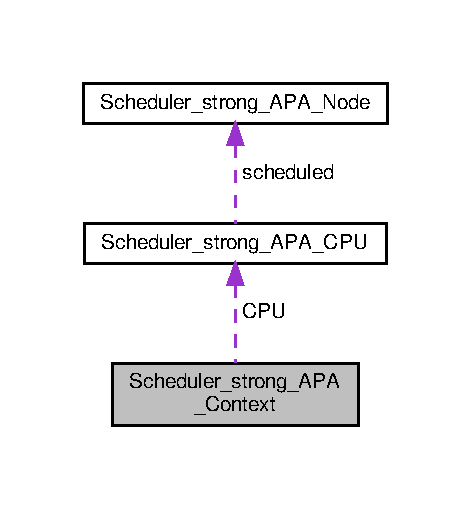
\includegraphics[width=226pt]{structScheduler__strong__APA__Context__coll__graph}
\end{center}
\end{figure}
\subsection*{Public Attributes}
\begin{DoxyCompactItemize}
\item 
Scheduler\+\_\+\+S\+M\+P\+\_\+\+Context \hyperlink{structScheduler__strong__APA__Context_a55755b445b7e7beaf1b87b178521e615}{Base}
\begin{DoxyCompactList}\small\item\em S\+MP Context to refer to S\+MP implementation code. \end{DoxyCompactList}\item 
\hyperlink{structScheduler__strong__APA__CPU}{Scheduler\+\_\+strong\+\_\+\+A\+P\+A\+\_\+\+C\+PU} \hyperlink{structScheduler__strong__APA__Context_afdc7dcc1fef07a07130a8ddde0895e9c}{C\+PU} \mbox{[}R\+T\+E\+M\+S\+\_\+\+Z\+E\+R\+O\+\_\+\+L\+E\+N\+G\+T\+H\+\_\+\+A\+R\+R\+AY\mbox{]}
\begin{DoxyCompactList}\small\item\em A table with structure for each C\+PU. \end{DoxyCompactList}\end{DoxyCompactItemize}


\subsection{Detailed Description}
Scheduler context for Strong A\+PA scheduler. 

Has the structure for scheduler context and Node defintion for Strong A\+PA scheduler 

Definition at line 61 of file schedulerstrongapa.\+h.



\subsection{Member Data Documentation}
\mbox{\Hypertarget{structScheduler__strong__APA__Context_a55755b445b7e7beaf1b87b178521e615}\label{structScheduler__strong__APA__Context_a55755b445b7e7beaf1b87b178521e615}} 
\index{Scheduler\+\_\+strong\+\_\+\+A\+P\+A\+\_\+\+Context@{Scheduler\+\_\+strong\+\_\+\+A\+P\+A\+\_\+\+Context}!Base@{Base}}
\index{Base@{Base}!Scheduler\+\_\+strong\+\_\+\+A\+P\+A\+\_\+\+Context@{Scheduler\+\_\+strong\+\_\+\+A\+P\+A\+\_\+\+Context}}
\subsubsection{\texorpdfstring{Base}{Base}}
{\footnotesize\ttfamily Scheduler\+\_\+\+S\+M\+P\+\_\+\+Context Scheduler\+\_\+strong\+\_\+\+A\+P\+A\+\_\+\+Context\+::\+Base}



S\+MP Context to refer to S\+MP implementation code. 



Definition at line 66 of file schedulerstrongapa.\+h.

\mbox{\Hypertarget{structScheduler__strong__APA__Context_afdc7dcc1fef07a07130a8ddde0895e9c}\label{structScheduler__strong__APA__Context_afdc7dcc1fef07a07130a8ddde0895e9c}} 
\index{Scheduler\+\_\+strong\+\_\+\+A\+P\+A\+\_\+\+Context@{Scheduler\+\_\+strong\+\_\+\+A\+P\+A\+\_\+\+Context}!C\+PU@{C\+PU}}
\index{C\+PU@{C\+PU}!Scheduler\+\_\+strong\+\_\+\+A\+P\+A\+\_\+\+Context@{Scheduler\+\_\+strong\+\_\+\+A\+P\+A\+\_\+\+Context}}
\subsubsection{\texorpdfstring{C\+PU}{CPU}}
{\footnotesize\ttfamily \hyperlink{structScheduler__strong__APA__CPU}{Scheduler\+\_\+strong\+\_\+\+A\+P\+A\+\_\+\+C\+PU} Scheduler\+\_\+strong\+\_\+\+A\+P\+A\+\_\+\+Context\+::\+C\+PU\mbox{[}R\+T\+E\+M\+S\+\_\+\+Z\+E\+R\+O\+\_\+\+L\+E\+N\+G\+T\+H\+\_\+\+A\+R\+R\+AY\mbox{]}}



A table with structure for each C\+PU. 

The index correspond to the C\+PU index, so index 0 points to C\+PU 0 and so on. 

Definition at line 74 of file schedulerstrongapa.\+h.



The documentation for this struct was generated from the following file\+:\begin{DoxyCompactItemize}
\item 
\hyperlink{schedulerstrongapa_8h}{schedulerstrongapa.\+h}\end{DoxyCompactItemize}

\hypertarget{structScheduler__strong__APA__Node}{}\section{Scheduler\+\_\+strong\+\_\+\+A\+P\+A\+\_\+\+Node Struct Reference}
\label{structScheduler__strong__APA__Node}\index{Scheduler\+\_\+strong\+\_\+\+A\+P\+A\+\_\+\+Node@{Scheduler\+\_\+strong\+\_\+\+A\+P\+A\+\_\+\+Node}}


Scheduler node specialization for Strong A\+PA schedulers.  




{\ttfamily \#include $<$schedulerstrongapa.\+h$>$}

\subsection*{Public Attributes}
\begin{DoxyCompactItemize}
\item 
Scheduler\+\_\+\+S\+M\+P\+\_\+\+Node \hyperlink{structScheduler__strong__APA__Node_ae86cbf5fd8743267abe33bed6d8b0fe6}{Base}
\begin{DoxyCompactList}\small\item\em S\+MP scheduler node. \end{DoxyCompactList}\item 
Processor\+\_\+mask \hyperlink{structScheduler__strong__APA__Node_a2e8928b11f1738a11c228780eb849989}{affinity}
\begin{DoxyCompactList}\small\item\em The associated affinity set of this node. \end{DoxyCompactList}\end{DoxyCompactItemize}


\subsection{Detailed Description}
Scheduler node specialization for Strong A\+PA schedulers. 

Definition at line 75 of file schedulerstrongapa.\+h.



\subsection{Member Data Documentation}
\mbox{\Hypertarget{structScheduler__strong__APA__Node_a2e8928b11f1738a11c228780eb849989}\label{structScheduler__strong__APA__Node_a2e8928b11f1738a11c228780eb849989}} 
\index{Scheduler\+\_\+strong\+\_\+\+A\+P\+A\+\_\+\+Node@{Scheduler\+\_\+strong\+\_\+\+A\+P\+A\+\_\+\+Node}!affinity@{affinity}}
\index{affinity@{affinity}!Scheduler\+\_\+strong\+\_\+\+A\+P\+A\+\_\+\+Node@{Scheduler\+\_\+strong\+\_\+\+A\+P\+A\+\_\+\+Node}}
\subsubsection{\texorpdfstring{affinity}{affinity}}
{\footnotesize\ttfamily Processor\+\_\+mask Scheduler\+\_\+strong\+\_\+\+A\+P\+A\+\_\+\+Node\+::affinity}



The associated affinity set of this node. 



Definition at line 84 of file schedulerstrongapa.\+h.

\mbox{\Hypertarget{structScheduler__strong__APA__Node_ae86cbf5fd8743267abe33bed6d8b0fe6}\label{structScheduler__strong__APA__Node_ae86cbf5fd8743267abe33bed6d8b0fe6}} 
\index{Scheduler\+\_\+strong\+\_\+\+A\+P\+A\+\_\+\+Node@{Scheduler\+\_\+strong\+\_\+\+A\+P\+A\+\_\+\+Node}!Base@{Base}}
\index{Base@{Base}!Scheduler\+\_\+strong\+\_\+\+A\+P\+A\+\_\+\+Node@{Scheduler\+\_\+strong\+\_\+\+A\+P\+A\+\_\+\+Node}}
\subsubsection{\texorpdfstring{Base}{Base}}
{\footnotesize\ttfamily Scheduler\+\_\+\+S\+M\+P\+\_\+\+Node Scheduler\+\_\+strong\+\_\+\+A\+P\+A\+\_\+\+Node\+::\+Base}



S\+MP scheduler node. 



Definition at line 79 of file schedulerstrongapa.\+h.



The documentation for this struct was generated from the following file\+:\begin{DoxyCompactItemize}
\item 
\hyperlink{schedulerstrongapa_8h}{schedulerstrongapa.\+h}\end{DoxyCompactItemize}

\hypertarget{structScheduler__strong__APA__Struct}{}\section{Scheduler\+\_\+strong\+\_\+\+A\+P\+A\+\_\+\+Struct Struct Reference}
\label{structScheduler__strong__APA__Struct}\index{Scheduler\+\_\+strong\+\_\+\+A\+P\+A\+\_\+\+Struct@{Scheduler\+\_\+strong\+\_\+\+A\+P\+A\+\_\+\+Struct}}


Struct for each index of the variable size arrays.  




{\ttfamily \#include $<$schedulerstrongapa.\+h$>$}

\subsection*{Public Attributes}
\begin{DoxyCompactItemize}
\item 
Scheduler\+\_\+\+Node $\ast$ \hyperlink{structScheduler__strong__APA__Struct_a9ab1e221dcee9eaebb131158da9a338e}{caller}
\begin{DoxyCompactList}\small\item\em The node that called this C\+PU, i.\+e. \end{DoxyCompactList}\item 
Per\+\_\+\+C\+P\+U\+\_\+\+Control $\ast$ \hyperlink{structScheduler__strong__APA__Struct_a83534c31f08a040a5a24b48007f17a09}{cpu}
\begin{DoxyCompactList}\small\item\em Cpu at the index of \hyperlink{structScheduler__strong__APA__Context_ac25debff84510636df8e42c5750ace15}{Scheduler\+\_\+strong\+\_\+\+A\+P\+A\+\_\+\+Context\+::\+Struct} in Queue implementation. \end{DoxyCompactList}\item 
bool \hyperlink{structScheduler__strong__APA__Struct_ab611e883dcef8c5226f00c734876b132}{visited}
\begin{DoxyCompactList}\small\item\em Indicates if the C\+PU at the index of \hyperlink{structScheduler__strong__APA__Context_ac25debff84510636df8e42c5750ace15}{Scheduler\+\_\+strong\+\_\+\+A\+P\+A\+\_\+\+Context\+::\+Struct} is already added to the Queue or not. \end{DoxyCompactList}\end{DoxyCompactItemize}


\subsection{Detailed Description}
Struct for each index of the variable size arrays. 

Definition at line 90 of file schedulerstrongapa.\+h.



\subsection{Member Data Documentation}
\mbox{\Hypertarget{structScheduler__strong__APA__Struct_a9ab1e221dcee9eaebb131158da9a338e}\label{structScheduler__strong__APA__Struct_a9ab1e221dcee9eaebb131158da9a338e}} 
\index{Scheduler\+\_\+strong\+\_\+\+A\+P\+A\+\_\+\+Struct@{Scheduler\+\_\+strong\+\_\+\+A\+P\+A\+\_\+\+Struct}!caller@{caller}}
\index{caller@{caller}!Scheduler\+\_\+strong\+\_\+\+A\+P\+A\+\_\+\+Struct@{Scheduler\+\_\+strong\+\_\+\+A\+P\+A\+\_\+\+Struct}}
\subsubsection{\texorpdfstring{caller}{caller}}
{\footnotesize\ttfamily Scheduler\+\_\+\+Node$\ast$ Scheduler\+\_\+strong\+\_\+\+A\+P\+A\+\_\+\+Struct\+::caller}



The node that called this C\+PU, i.\+e. 

a node which has the cpu at the index of \hyperlink{structScheduler__strong__APA__Context_ac25debff84510636df8e42c5750ace15}{Scheduler\+\_\+strong\+\_\+\+A\+P\+A\+\_\+\+Context\+::\+Struct} in its affinity set. 

Definition at line 97 of file schedulerstrongapa.\+h.

\mbox{\Hypertarget{structScheduler__strong__APA__Struct_a83534c31f08a040a5a24b48007f17a09}\label{structScheduler__strong__APA__Struct_a83534c31f08a040a5a24b48007f17a09}} 
\index{Scheduler\+\_\+strong\+\_\+\+A\+P\+A\+\_\+\+Struct@{Scheduler\+\_\+strong\+\_\+\+A\+P\+A\+\_\+\+Struct}!cpu@{cpu}}
\index{cpu@{cpu}!Scheduler\+\_\+strong\+\_\+\+A\+P\+A\+\_\+\+Struct@{Scheduler\+\_\+strong\+\_\+\+A\+P\+A\+\_\+\+Struct}}
\subsubsection{\texorpdfstring{cpu}{cpu}}
{\footnotesize\ttfamily Per\+\_\+\+C\+P\+U\+\_\+\+Control$\ast$ Scheduler\+\_\+strong\+\_\+\+A\+P\+A\+\_\+\+Struct\+::cpu}



Cpu at the index of \hyperlink{structScheduler__strong__APA__Context_ac25debff84510636df8e42c5750ace15}{Scheduler\+\_\+strong\+\_\+\+A\+P\+A\+\_\+\+Context\+::\+Struct} in Queue implementation. 



Definition at line 103 of file schedulerstrongapa.\+h.

\mbox{\Hypertarget{structScheduler__strong__APA__Struct_ab611e883dcef8c5226f00c734876b132}\label{structScheduler__strong__APA__Struct_ab611e883dcef8c5226f00c734876b132}} 
\index{Scheduler\+\_\+strong\+\_\+\+A\+P\+A\+\_\+\+Struct@{Scheduler\+\_\+strong\+\_\+\+A\+P\+A\+\_\+\+Struct}!visited@{visited}}
\index{visited@{visited}!Scheduler\+\_\+strong\+\_\+\+A\+P\+A\+\_\+\+Struct@{Scheduler\+\_\+strong\+\_\+\+A\+P\+A\+\_\+\+Struct}}
\subsubsection{\texorpdfstring{visited}{visited}}
{\footnotesize\ttfamily bool Scheduler\+\_\+strong\+\_\+\+A\+P\+A\+\_\+\+Struct\+::visited}



Indicates if the C\+PU at the index of \hyperlink{structScheduler__strong__APA__Context_ac25debff84510636df8e42c5750ace15}{Scheduler\+\_\+strong\+\_\+\+A\+P\+A\+\_\+\+Context\+::\+Struct} is already added to the Queue or not. 



Definition at line 110 of file schedulerstrongapa.\+h.



The documentation for this struct was generated from the following file\+:\begin{DoxyCompactItemize}
\item 
\hyperlink{schedulerstrongapa_8h}{schedulerstrongapa.\+h}\end{DoxyCompactItemize}

\chapter{File Documentation}
\hypertarget{mainpage_8dox}{}\section{mainpage.\+dox File Reference}
\label{mainpage_8dox}\index{mainpage.\+dox@{mainpage.\+dox}}

\hypertarget{schedulerstrongapa_8c}{}\section{schedulerstrongapa.\+c File Reference}
\label{schedulerstrongapa_8c}\index{schedulerstrongapa.\+c@{schedulerstrongapa.\+c}}
\subsection*{Functions}
\begin{DoxyCompactItemize}
\item 
void \hyperlink{schedulerstrongapa_8c_afcd6fde337d7542784698219322b6365}{\+\_\+\+Scheduler\+\_\+strong\+\_\+\+A\+P\+A\+\_\+\+Initialize} (const Scheduler\+\_\+\+Control $\ast$scheduler)
\begin{DoxyCompactList}\small\item\em Initializes the Strong\+\_\+\+A\+PA scheduler. \end{DoxyCompactList}\item 
void \hyperlink{group__RTEMSScoreSchedulerStrongAPA_ga1cde4345d4dc0b5a37a696fa446bb47e}{\+\_\+\+Scheduler\+\_\+strong\+\_\+\+A\+P\+A\+\_\+\+Node\+\_\+initialize} (const Scheduler\+\_\+\+Control $\ast$scheduler, Scheduler\+\_\+\+Node $\ast$node, Thread\+\_\+\+Control $\ast$the\+\_\+thread, Priority\+\_\+\+Control priority)
\begin{DoxyCompactList}\small\item\em Initializes the node with the given priority. \end{DoxyCompactList}\item 
bool \hyperlink{schedulerstrongapa_8c_a63ef624a9881cf77a2b1eef2c6f05223}{\+\_\+\+Scheduler\+\_\+strong\+\_\+\+A\+P\+A\+\_\+\+Set\+\_\+affinity} (const Scheduler\+\_\+\+Control $\ast$scheduler, Thread\+\_\+\+Control $\ast$thread, Scheduler\+\_\+\+Node $\ast$node\+\_\+base, const Processor\+\_\+mask $\ast$affinity)
\end{DoxyCompactItemize}
\subsection*{Variables}
\begin{DoxyCompactItemize}
\item 
To\+Add \hyperlink{schedulerstrongapa_8c_a72fea2084c662e7ee54c4ec79afa6cb1}{\+\_\+\+\_\+pad0\+\_\+\+\_\+}
\item 
To\+Add \hyperlink{schedulerstrongapa_8c_a8945ef8d0eb337a3b389f45209054a49}{\+\_\+\+Scheduler\+\_\+default\+\_\+\+Schedule}
\item 
To\+Add \hyperlink{schedulerstrongapa_8c_a1f51bd961a796a572919fafc709dd11f}{\+\_\+\+Scheduler\+\_\+strong\+\_\+\+A\+P\+A\+\_\+\+Yield}
\item 
To\+Add \hyperlink{schedulerstrongapa_8c_a77b4dcee45205dd5e72addfa921af4cc}{\+\_\+\+Scheduler\+\_\+strong\+\_\+\+A\+P\+A\+\_\+\+Block}
\item 
To\+Add \hyperlink{schedulerstrongapa_8c_a81baa0f3613f9b9d8cc2cbf937cf57cd}{\+\_\+\+Scheduler\+\_\+strong\+\_\+\+A\+P\+A\+\_\+\+Unblock}
\item 
To\+Add \hyperlink{schedulerstrongapa_8c_a9c87b05d6ee253bf3dbc583c17654456}{\+\_\+\+Scheduler\+\_\+strong\+\_\+\+A\+P\+A\+\_\+\+Update\+\_\+priority}
\item 
To\+Add \hyperlink{schedulerstrongapa_8c_aca2acd0295cd7ed2ea2d4d3720dd9486}{\+\_\+\+Scheduler\+\_\+default\+\_\+\+Map\+\_\+priority}
\item 
To\+Add \hyperlink{schedulerstrongapa_8c_af764b1eb60937d5cb4b12cdae7ffc931}{\+\_\+\+Scheduler\+\_\+default\+\_\+\+Unmap\+\_\+priority}
\item 
To\+Add \hyperlink{schedulerstrongapa_8c_ae918381ccf0f7d0c5d88e7603a7a1aea}{\+\_\+\+Scheduler\+\_\+strong\+\_\+\+A\+P\+A\+\_\+\+Ask\+\_\+for\+\_\+help}
\item 
To\+Add \hyperlink{schedulerstrongapa_8c_a27be05a567ea574c74a30f5baf8b1a28}{\+\_\+\+Scheduler\+\_\+strong\+\_\+\+A\+P\+A\+\_\+\+Reconsider\+\_\+help\+\_\+request}
\item 
To\+Add \hyperlink{schedulerstrongapa_8c_a51496fdfb596c6b2eb2c3beafa7d39d8}{\+\_\+\+Scheduler\+\_\+strong\+\_\+\+A\+P\+A\+\_\+\+Withdraw\+\_\+node}
\item 
To\+Add \hyperlink{schedulerstrongapa_8c_a0ba8ebe2b0b7eaa855e8eea83fb48b49}{\+\_\+\+Scheduler\+\_\+default\+\_\+\+Pin\+\_\+or\+\_\+unpin}
\item 
To\+Add \hyperlink{schedulerstrongapa_8c_a4fd003aab858ebba4664fa5934368385}{\+\_\+\+Scheduler\+\_\+strong\+\_\+\+A\+P\+A\+\_\+\+Add\+\_\+processor}
\item 
To\+Add \hyperlink{schedulerstrongapa_8c_a6d189bb139fa6f6c1f65a9244178412b}{\+\_\+\+Scheduler\+\_\+strong\+\_\+\+A\+P\+A\+\_\+\+Remove\+\_\+processor}
\item 
To\+Add \hyperlink{schedulerstrongapa_8c_ac6ed869799a85c0f29252a85d9ef3541}{\+\_\+\+Scheduler\+\_\+strong\+\_\+\+A\+P\+A\+\_\+\+Node\+\_\+initialize}
\item 
To\+Add \hyperlink{schedulerstrongapa_8c_ab6186ad9eeef16e5869ab59d382edc34}{\+\_\+\+Scheduler\+\_\+default\+\_\+\+Node\+\_\+destroy}
\item 
To\+Add \hyperlink{schedulerstrongapa_8c_a5b6a590129571341b8e96158d8dfa7c9}{\+\_\+\+Scheduler\+\_\+default\+\_\+\+Release\+\_\+job}
\item 
To\+Add \hyperlink{schedulerstrongapa_8c_a5aece934fec118dcad2eaa15010fa22d}{\+\_\+\+Scheduler\+\_\+default\+\_\+\+Cancel\+\_\+job}
\item 
To\+Add \hyperlink{schedulerstrongapa_8c_a304c1170091ec720ca05bb3960df127e}{\+\_\+\+Scheduler\+\_\+default\+\_\+\+Tick}
\item 
To\+Add \+\_\+\+Scheduler\+\_\+\+S\+M\+P\+\_\+\+Start\+\_\+idle \hyperlink{schedulerstrongapa_8c_a63ef624a9881cf77a2b1eef2c6f05223}{\+\_\+\+Scheduler\+\_\+strong\+\_\+\+A\+P\+A\+\_\+\+Set\+\_\+affinity} S\+C\+H\+E\+D\+U\+L\+E\+R\+\_\+\+O\+P\+E\+R\+A\+T\+I\+O\+N\+\_\+\+D\+E\+F\+A\+U\+L\+T\+\_\+\+G\+E\+T\+\_\+\+S\+E\+T\+\_\+\+A\+F\+F\+I\+N\+I\+TY Refer from \hyperlink{schedulerstrongapa_8c_abbd4c925f1ad59918c1f68bf8f489913}{\+\_\+\+Scheduler\+\_\+\+E\+D\+F\+\_\+\+S\+M\+P\+\_\+\+Initialize}
\item 
To\+Add \+\_\+\+Scheduler\+\_\+\+S\+M\+P\+\_\+\+Start\+\_\+idle \hyperlink{schedulerstrongapa_8c_a63ef624a9881cf77a2b1eef2c6f05223}{\+\_\+\+Scheduler\+\_\+strong\+\_\+\+A\+P\+A\+\_\+\+Set\+\_\+affinity} S\+C\+H\+E\+D\+U\+L\+E\+R\+\_\+\+O\+P\+E\+R\+A\+T\+I\+O\+N\+\_\+\+D\+E\+F\+A\+U\+L\+T\+\_\+\+G\+E\+T\+\_\+\+S\+E\+T\+\_\+\+A\+F\+F\+I\+N\+I\+TY Refer from \hyperlink{schedulerstrongapa_8c_a077109cb201338a365b3d0c2c7bd61ee}{\+\_\+\+Scheduler\+\_\+\+E\+D\+F\+\_\+\+S\+M\+P\+\_\+\+Yield}
\item 
To\+Add \+\_\+\+Scheduler\+\_\+\+S\+M\+P\+\_\+\+Start\+\_\+idle \hyperlink{schedulerstrongapa_8c_a63ef624a9881cf77a2b1eef2c6f05223}{\+\_\+\+Scheduler\+\_\+strong\+\_\+\+A\+P\+A\+\_\+\+Set\+\_\+affinity} S\+C\+H\+E\+D\+U\+L\+E\+R\+\_\+\+O\+P\+E\+R\+A\+T\+I\+O\+N\+\_\+\+D\+E\+F\+A\+U\+L\+T\+\_\+\+G\+E\+T\+\_\+\+S\+E\+T\+\_\+\+A\+F\+F\+I\+N\+I\+TY Refer from \hyperlink{schedulerstrongapa_8c_ae690d490e9de7a40d13681bc5b398cec}{\+\_\+\+Scheduler\+\_\+\+E\+D\+F\+\_\+\+S\+M\+P\+\_\+\+Block}
\item 
To\+Add \+\_\+\+Scheduler\+\_\+\+S\+M\+P\+\_\+\+Start\+\_\+idle \hyperlink{schedulerstrongapa_8c_a63ef624a9881cf77a2b1eef2c6f05223}{\+\_\+\+Scheduler\+\_\+strong\+\_\+\+A\+P\+A\+\_\+\+Set\+\_\+affinity} S\+C\+H\+E\+D\+U\+L\+E\+R\+\_\+\+O\+P\+E\+R\+A\+T\+I\+O\+N\+\_\+\+D\+E\+F\+A\+U\+L\+T\+\_\+\+G\+E\+T\+\_\+\+S\+E\+T\+\_\+\+A\+F\+F\+I\+N\+I\+TY Refer from \hyperlink{schedulerstrongapa_8c_aead352606a75abc7e2f3f065698810a5}{\+\_\+\+Scheduler\+\_\+\+E\+D\+F\+\_\+\+S\+M\+P\+\_\+\+Unblock}
\item 
To\+Add \+\_\+\+Scheduler\+\_\+\+S\+M\+P\+\_\+\+Start\+\_\+idle \hyperlink{schedulerstrongapa_8c_a63ef624a9881cf77a2b1eef2c6f05223}{\+\_\+\+Scheduler\+\_\+strong\+\_\+\+A\+P\+A\+\_\+\+Set\+\_\+affinity} S\+C\+H\+E\+D\+U\+L\+E\+R\+\_\+\+O\+P\+E\+R\+A\+T\+I\+O\+N\+\_\+\+D\+E\+F\+A\+U\+L\+T\+\_\+\+G\+E\+T\+\_\+\+S\+E\+T\+\_\+\+A\+F\+F\+I\+N\+I\+TY Refer from \hyperlink{schedulerstrongapa_8c_a7b35749ff23972ad0616c8bd633e2ce6}{\+\_\+\+Scheduler\+\_\+\+E\+D\+F\+\_\+\+S\+M\+P\+\_\+\+Update\+\_\+priority}
\item 
To\+Add \+\_\+\+Scheduler\+\_\+\+S\+M\+P\+\_\+\+Start\+\_\+idle \hyperlink{schedulerstrongapa_8c_a63ef624a9881cf77a2b1eef2c6f05223}{\+\_\+\+Scheduler\+\_\+strong\+\_\+\+A\+P\+A\+\_\+\+Set\+\_\+affinity} S\+C\+H\+E\+D\+U\+L\+E\+R\+\_\+\+O\+P\+E\+R\+A\+T\+I\+O\+N\+\_\+\+D\+E\+F\+A\+U\+L\+T\+\_\+\+G\+E\+T\+\_\+\+S\+E\+T\+\_\+\+A\+F\+F\+I\+N\+I\+TY Refer from \hyperlink{schedulerstrongapa_8c_a2769f601d34ccb09fccf0a2cd00d8fa1}{\+\_\+\+Scheduler\+\_\+\+E\+D\+F\+\_\+\+Map\+\_\+priority}
\item 
To\+Add \+\_\+\+Scheduler\+\_\+\+S\+M\+P\+\_\+\+Start\+\_\+idle \hyperlink{schedulerstrongapa_8c_a63ef624a9881cf77a2b1eef2c6f05223}{\+\_\+\+Scheduler\+\_\+strong\+\_\+\+A\+P\+A\+\_\+\+Set\+\_\+affinity} S\+C\+H\+E\+D\+U\+L\+E\+R\+\_\+\+O\+P\+E\+R\+A\+T\+I\+O\+N\+\_\+\+D\+E\+F\+A\+U\+L\+T\+\_\+\+G\+E\+T\+\_\+\+S\+E\+T\+\_\+\+A\+F\+F\+I\+N\+I\+TY Refer from \hyperlink{schedulerstrongapa_8c_aefc6b9a6b1aec14a71fe80a163095313}{\+\_\+\+Scheduler\+\_\+\+E\+D\+F\+\_\+\+Unmap\+\_\+priority}
\item 
To\+Add \+\_\+\+Scheduler\+\_\+\+S\+M\+P\+\_\+\+Start\+\_\+idle \hyperlink{schedulerstrongapa_8c_a63ef624a9881cf77a2b1eef2c6f05223}{\+\_\+\+Scheduler\+\_\+strong\+\_\+\+A\+P\+A\+\_\+\+Set\+\_\+affinity} S\+C\+H\+E\+D\+U\+L\+E\+R\+\_\+\+O\+P\+E\+R\+A\+T\+I\+O\+N\+\_\+\+D\+E\+F\+A\+U\+L\+T\+\_\+\+G\+E\+T\+\_\+\+S\+E\+T\+\_\+\+A\+F\+F\+I\+N\+I\+TY Refer from \hyperlink{schedulerstrongapa_8c_a456dbdfe2e595c0f38c03e6d7b2ab938}{\+\_\+\+Scheduler\+\_\+\+E\+D\+F\+\_\+\+S\+M\+P\+\_\+\+Ask\+\_\+for\+\_\+help}
\item 
To\+Add \+\_\+\+Scheduler\+\_\+\+S\+M\+P\+\_\+\+Start\+\_\+idle \hyperlink{schedulerstrongapa_8c_a63ef624a9881cf77a2b1eef2c6f05223}{\+\_\+\+Scheduler\+\_\+strong\+\_\+\+A\+P\+A\+\_\+\+Set\+\_\+affinity} S\+C\+H\+E\+D\+U\+L\+E\+R\+\_\+\+O\+P\+E\+R\+A\+T\+I\+O\+N\+\_\+\+D\+E\+F\+A\+U\+L\+T\+\_\+\+G\+E\+T\+\_\+\+S\+E\+T\+\_\+\+A\+F\+F\+I\+N\+I\+TY Refer from \hyperlink{schedulerstrongapa_8c_a99dabbee6249603b4e542e23b7d46457}{\+\_\+\+Scheduler\+\_\+\+E\+D\+F\+\_\+\+S\+M\+P\+\_\+\+Reconsider\+\_\+help\+\_\+request}
\item 
To\+Add \+\_\+\+Scheduler\+\_\+\+S\+M\+P\+\_\+\+Start\+\_\+idle \hyperlink{schedulerstrongapa_8c_a63ef624a9881cf77a2b1eef2c6f05223}{\+\_\+\+Scheduler\+\_\+strong\+\_\+\+A\+P\+A\+\_\+\+Set\+\_\+affinity} S\+C\+H\+E\+D\+U\+L\+E\+R\+\_\+\+O\+P\+E\+R\+A\+T\+I\+O\+N\+\_\+\+D\+E\+F\+A\+U\+L\+T\+\_\+\+G\+E\+T\+\_\+\+S\+E\+T\+\_\+\+A\+F\+F\+I\+N\+I\+TY Refer from \hyperlink{schedulerstrongapa_8c_ae45c93d4fac4a7ad988f8e469773da04}{\+\_\+\+Scheduler\+\_\+\+E\+D\+F\+\_\+\+S\+M\+P\+\_\+\+Withdraw\+\_\+node}
\item 
To\+Add \+\_\+\+Scheduler\+\_\+\+S\+M\+P\+\_\+\+Start\+\_\+idle \hyperlink{schedulerstrongapa_8c_a63ef624a9881cf77a2b1eef2c6f05223}{\+\_\+\+Scheduler\+\_\+strong\+\_\+\+A\+P\+A\+\_\+\+Set\+\_\+affinity} S\+C\+H\+E\+D\+U\+L\+E\+R\+\_\+\+O\+P\+E\+R\+A\+T\+I\+O\+N\+\_\+\+D\+E\+F\+A\+U\+L\+T\+\_\+\+G\+E\+T\+\_\+\+S\+E\+T\+\_\+\+A\+F\+F\+I\+N\+I\+TY Refer from \hyperlink{schedulerstrongapa_8c_aac7fff4c1d9b04e5f36109a01673f2d9}{\+\_\+\+Scheduler\+\_\+\+E\+D\+F\+\_\+\+S\+M\+P\+\_\+\+Pin}
\item 
To\+Add \+\_\+\+Scheduler\+\_\+\+S\+M\+P\+\_\+\+Start\+\_\+idle \hyperlink{schedulerstrongapa_8c_a63ef624a9881cf77a2b1eef2c6f05223}{\+\_\+\+Scheduler\+\_\+strong\+\_\+\+A\+P\+A\+\_\+\+Set\+\_\+affinity} S\+C\+H\+E\+D\+U\+L\+E\+R\+\_\+\+O\+P\+E\+R\+A\+T\+I\+O\+N\+\_\+\+D\+E\+F\+A\+U\+L\+T\+\_\+\+G\+E\+T\+\_\+\+S\+E\+T\+\_\+\+A\+F\+F\+I\+N\+I\+TY Refer from \hyperlink{schedulerstrongapa_8c_af785e560c9f14bd1e487f2da466b59c6}{\+\_\+\+Scheduler\+\_\+\+E\+D\+F\+\_\+\+S\+M\+P\+\_\+\+Unpin}
\item 
To\+Add \+\_\+\+Scheduler\+\_\+\+S\+M\+P\+\_\+\+Start\+\_\+idle \hyperlink{schedulerstrongapa_8c_a63ef624a9881cf77a2b1eef2c6f05223}{\+\_\+\+Scheduler\+\_\+strong\+\_\+\+A\+P\+A\+\_\+\+Set\+\_\+affinity} S\+C\+H\+E\+D\+U\+L\+E\+R\+\_\+\+O\+P\+E\+R\+A\+T\+I\+O\+N\+\_\+\+D\+E\+F\+A\+U\+L\+T\+\_\+\+G\+E\+T\+\_\+\+S\+E\+T\+\_\+\+A\+F\+F\+I\+N\+I\+TY Refer from \hyperlink{schedulerstrongapa_8c_aac408c0e93dc1a7429c49afc315627a0}{\+\_\+\+Scheduler\+\_\+\+E\+D\+F\+\_\+\+S\+M\+P\+\_\+\+Add\+\_\+processor}
\item 
To\+Add \+\_\+\+Scheduler\+\_\+\+S\+M\+P\+\_\+\+Start\+\_\+idle \hyperlink{schedulerstrongapa_8c_a63ef624a9881cf77a2b1eef2c6f05223}{\+\_\+\+Scheduler\+\_\+strong\+\_\+\+A\+P\+A\+\_\+\+Set\+\_\+affinity} S\+C\+H\+E\+D\+U\+L\+E\+R\+\_\+\+O\+P\+E\+R\+A\+T\+I\+O\+N\+\_\+\+D\+E\+F\+A\+U\+L\+T\+\_\+\+G\+E\+T\+\_\+\+S\+E\+T\+\_\+\+A\+F\+F\+I\+N\+I\+TY Refer from \hyperlink{schedulerstrongapa_8c_ae4bec75ee6a51c8a3220941d24f43c79}{\+\_\+\+Scheduler\+\_\+\+E\+D\+F\+\_\+\+S\+M\+P\+\_\+\+Remove\+\_\+processor}
\item 
To\+Add \+\_\+\+Scheduler\+\_\+\+S\+M\+P\+\_\+\+Start\+\_\+idle \hyperlink{schedulerstrongapa_8c_a63ef624a9881cf77a2b1eef2c6f05223}{\+\_\+\+Scheduler\+\_\+strong\+\_\+\+A\+P\+A\+\_\+\+Set\+\_\+affinity} S\+C\+H\+E\+D\+U\+L\+E\+R\+\_\+\+O\+P\+E\+R\+A\+T\+I\+O\+N\+\_\+\+D\+E\+F\+A\+U\+L\+T\+\_\+\+G\+E\+T\+\_\+\+S\+E\+T\+\_\+\+A\+F\+F\+I\+N\+I\+TY Refer from \hyperlink{schedulerstrongapa_8c_ad9c6d0d77accc70d1b188ba5d5f966d3}{\+\_\+\+Scheduler\+\_\+\+E\+D\+F\+\_\+\+S\+M\+P\+\_\+\+Node\+\_\+initialize}
\item 
To\+Add \+\_\+\+Scheduler\+\_\+\+S\+M\+P\+\_\+\+Start\+\_\+idle \hyperlink{schedulerstrongapa_8c_a63ef624a9881cf77a2b1eef2c6f05223}{\+\_\+\+Scheduler\+\_\+strong\+\_\+\+A\+P\+A\+\_\+\+Set\+\_\+affinity} S\+C\+H\+E\+D\+U\+L\+E\+R\+\_\+\+O\+P\+E\+R\+A\+T\+I\+O\+N\+\_\+\+D\+E\+F\+A\+U\+L\+T\+\_\+\+G\+E\+T\+\_\+\+S\+E\+T\+\_\+\+A\+F\+F\+I\+N\+I\+TY Refer from \hyperlink{schedulerstrongapa_8c_a519b4f6f7947b339b24550e356db057e}{\+\_\+\+Scheduler\+\_\+\+E\+D\+F\+\_\+\+Release\+\_\+job}
\item 
To\+Add \+\_\+\+Scheduler\+\_\+\+S\+M\+P\+\_\+\+Start\+\_\+idle \hyperlink{schedulerstrongapa_8c_a63ef624a9881cf77a2b1eef2c6f05223}{\+\_\+\+Scheduler\+\_\+strong\+\_\+\+A\+P\+A\+\_\+\+Set\+\_\+affinity} S\+C\+H\+E\+D\+U\+L\+E\+R\+\_\+\+O\+P\+E\+R\+A\+T\+I\+O\+N\+\_\+\+D\+E\+F\+A\+U\+L\+T\+\_\+\+G\+E\+T\+\_\+\+S\+E\+T\+\_\+\+A\+F\+F\+I\+N\+I\+TY Refer from \hyperlink{schedulerstrongapa_8c_a0f3d889050cdc7ceb482822c5e31c0ce}{\+\_\+\+Scheduler\+\_\+\+E\+D\+F\+\_\+\+Cancel\+\_\+job}
\item 
To\+Add \+\_\+\+Scheduler\+\_\+\+S\+M\+P\+\_\+\+Start\+\_\+idle \hyperlink{schedulerstrongapa_8c_a63ef624a9881cf77a2b1eef2c6f05223}{\+\_\+\+Scheduler\+\_\+strong\+\_\+\+A\+P\+A\+\_\+\+Set\+\_\+affinity} S\+C\+H\+E\+D\+U\+L\+E\+R\+\_\+\+O\+P\+E\+R\+A\+T\+I\+O\+N\+\_\+\+D\+E\+F\+A\+U\+L\+T\+\_\+\+G\+E\+T\+\_\+\+S\+E\+T\+\_\+\+A\+F\+F\+I\+N\+I\+TY Refer from \hyperlink{schedulerstrongapa_8c_a0f0df18acea3c0c29f214c36dc8aefe5}{\+\_\+\+Scheduler\+\_\+\+E\+D\+F\+\_\+\+S\+M\+P\+\_\+\+Start\+\_\+idle}
\end{DoxyCompactItemize}


\subsection{Function Documentation}
\mbox{\Hypertarget{schedulerstrongapa_8c_afcd6fde337d7542784698219322b6365}\label{schedulerstrongapa_8c_afcd6fde337d7542784698219322b6365}} 
\index{schedulerstrongapa.\+c@{schedulerstrongapa.\+c}!\+\_\+\+Scheduler\+\_\+strong\+\_\+\+A\+P\+A\+\_\+\+Initialize@{\+\_\+\+Scheduler\+\_\+strong\+\_\+\+A\+P\+A\+\_\+\+Initialize}}
\index{\+\_\+\+Scheduler\+\_\+strong\+\_\+\+A\+P\+A\+\_\+\+Initialize@{\+\_\+\+Scheduler\+\_\+strong\+\_\+\+A\+P\+A\+\_\+\+Initialize}!schedulerstrongapa.\+c@{schedulerstrongapa.\+c}}
\subsubsection{\texorpdfstring{\+\_\+\+Scheduler\+\_\+strong\+\_\+\+A\+P\+A\+\_\+\+Initialize()}{\_Scheduler\_strong\_APA\_Initialize()}}
{\footnotesize\ttfamily void \+\_\+\+Scheduler\+\_\+strong\+\_\+\+A\+P\+A\+\_\+\+Initialize (\begin{DoxyParamCaption}\item[{const Scheduler\+\_\+\+Control $\ast$}]{scheduler }\end{DoxyParamCaption})}



Initializes the Strong\+\_\+\+A\+PA scheduler. 

Sets the chain containing all the nodes to empty and initializes the S\+MP scheduler.


\begin{DoxyParams}{Parameters}
{\em scheduler} & used to get reference to Strong A\+PA scheduler context\\
\hline
\end{DoxyParams}
\begin{DoxyReturn}{Returns}
void
\end{DoxyReturn}
\begin{DoxySeeAlso}{See also}
\hyperlink{schedulerstrongapa_8c_ac6ed869799a85c0f29252a85d9ef3541}{\+\_\+\+Scheduler\+\_\+strong\+\_\+\+A\+P\+A\+\_\+\+Node\+\_\+initialize()} 
\end{DoxySeeAlso}


Definition at line 80 of file schedulerstrongapa.\+c.

\mbox{\Hypertarget{schedulerstrongapa_8c_a63ef624a9881cf77a2b1eef2c6f05223}\label{schedulerstrongapa_8c_a63ef624a9881cf77a2b1eef2c6f05223}} 
\index{schedulerstrongapa.\+c@{schedulerstrongapa.\+c}!\+\_\+\+Scheduler\+\_\+strong\+\_\+\+A\+P\+A\+\_\+\+Set\+\_\+affinity@{\+\_\+\+Scheduler\+\_\+strong\+\_\+\+A\+P\+A\+\_\+\+Set\+\_\+affinity}}
\index{\+\_\+\+Scheduler\+\_\+strong\+\_\+\+A\+P\+A\+\_\+\+Set\+\_\+affinity@{\+\_\+\+Scheduler\+\_\+strong\+\_\+\+A\+P\+A\+\_\+\+Set\+\_\+affinity}!schedulerstrongapa.\+c@{schedulerstrongapa.\+c}}
\subsubsection{\texorpdfstring{\+\_\+\+Scheduler\+\_\+strong\+\_\+\+A\+P\+A\+\_\+\+Set\+\_\+affinity()}{\_Scheduler\_strong\_APA\_Set\_affinity()}}
{\footnotesize\ttfamily bool \+\_\+\+Scheduler\+\_\+strong\+\_\+\+A\+P\+A\+\_\+\+Set\+\_\+affinity (\begin{DoxyParamCaption}\item[{const Scheduler\+\_\+\+Control $\ast$}]{scheduler,  }\item[{Thread\+\_\+\+Control $\ast$}]{thread,  }\item[{Scheduler\+\_\+\+Node $\ast$}]{node\+\_\+base,  }\item[{const Processor\+\_\+mask $\ast$}]{affinity }\end{DoxyParamCaption})}



Definition at line 124 of file schedulerstrongapa.\+c.



\subsection{Variable Documentation}
\mbox{\Hypertarget{schedulerstrongapa_8c_a72fea2084c662e7ee54c4ec79afa6cb1}\label{schedulerstrongapa_8c_a72fea2084c662e7ee54c4ec79afa6cb1}} 
\index{schedulerstrongapa.\+c@{schedulerstrongapa.\+c}!\+\_\+\+\_\+pad0\+\_\+\+\_\+@{\+\_\+\+\_\+pad0\+\_\+\+\_\+}}
\index{\+\_\+\+\_\+pad0\+\_\+\+\_\+@{\+\_\+\+\_\+pad0\+\_\+\+\_\+}!schedulerstrongapa.\+c@{schedulerstrongapa.\+c}}
\subsubsection{\texorpdfstring{\+\_\+\+\_\+pad0\+\_\+\+\_\+}{\_\_pad0\_\_}}
{\footnotesize\ttfamily To\+Add \+\_\+\+\_\+pad0\+\_\+\+\_\+}



Definition at line 3 of file schedulerstrongapa.\+c.

\mbox{\Hypertarget{schedulerstrongapa_8c_a5aece934fec118dcad2eaa15010fa22d}\label{schedulerstrongapa_8c_a5aece934fec118dcad2eaa15010fa22d}} 
\index{schedulerstrongapa.\+c@{schedulerstrongapa.\+c}!\+\_\+\+Scheduler\+\_\+default\+\_\+\+Cancel\+\_\+job@{\+\_\+\+Scheduler\+\_\+default\+\_\+\+Cancel\+\_\+job}}
\index{\+\_\+\+Scheduler\+\_\+default\+\_\+\+Cancel\+\_\+job@{\+\_\+\+Scheduler\+\_\+default\+\_\+\+Cancel\+\_\+job}!schedulerstrongapa.\+c@{schedulerstrongapa.\+c}}
\subsubsection{\texorpdfstring{\+\_\+\+Scheduler\+\_\+default\+\_\+\+Cancel\+\_\+job}{\_Scheduler\_default\_Cancel\_job}}
{\footnotesize\ttfamily To\+Add \+\_\+\+Scheduler\+\_\+default\+\_\+\+Cancel\+\_\+job}



Definition at line 3 of file schedulerstrongapa.\+c.

\mbox{\Hypertarget{schedulerstrongapa_8c_aca2acd0295cd7ed2ea2d4d3720dd9486}\label{schedulerstrongapa_8c_aca2acd0295cd7ed2ea2d4d3720dd9486}} 
\index{schedulerstrongapa.\+c@{schedulerstrongapa.\+c}!\+\_\+\+Scheduler\+\_\+default\+\_\+\+Map\+\_\+priority@{\+\_\+\+Scheduler\+\_\+default\+\_\+\+Map\+\_\+priority}}
\index{\+\_\+\+Scheduler\+\_\+default\+\_\+\+Map\+\_\+priority@{\+\_\+\+Scheduler\+\_\+default\+\_\+\+Map\+\_\+priority}!schedulerstrongapa.\+c@{schedulerstrongapa.\+c}}
\subsubsection{\texorpdfstring{\+\_\+\+Scheduler\+\_\+default\+\_\+\+Map\+\_\+priority}{\_Scheduler\_default\_Map\_priority}}
{\footnotesize\ttfamily To\+Add \+\_\+\+Scheduler\+\_\+default\+\_\+\+Map\+\_\+priority}



Definition at line 3 of file schedulerstrongapa.\+c.

\mbox{\Hypertarget{schedulerstrongapa_8c_ab6186ad9eeef16e5869ab59d382edc34}\label{schedulerstrongapa_8c_ab6186ad9eeef16e5869ab59d382edc34}} 
\index{schedulerstrongapa.\+c@{schedulerstrongapa.\+c}!\+\_\+\+Scheduler\+\_\+default\+\_\+\+Node\+\_\+destroy@{\+\_\+\+Scheduler\+\_\+default\+\_\+\+Node\+\_\+destroy}}
\index{\+\_\+\+Scheduler\+\_\+default\+\_\+\+Node\+\_\+destroy@{\+\_\+\+Scheduler\+\_\+default\+\_\+\+Node\+\_\+destroy}!schedulerstrongapa.\+c@{schedulerstrongapa.\+c}}
\subsubsection{\texorpdfstring{\+\_\+\+Scheduler\+\_\+default\+\_\+\+Node\+\_\+destroy}{\_Scheduler\_default\_Node\_destroy}}
{\footnotesize\ttfamily To\+Add \+\_\+\+Scheduler\+\_\+\+S\+M\+P\+\_\+\+Start\+\_\+idle \hyperlink{schedulerstrongapa_8c_a63ef624a9881cf77a2b1eef2c6f05223}{\+\_\+\+Scheduler\+\_\+strong\+\_\+\+A\+P\+A\+\_\+\+Set\+\_\+affinity} S\+C\+H\+E\+D\+U\+L\+E\+R\+\_\+\+O\+P\+E\+R\+A\+T\+I\+O\+N\+\_\+\+D\+E\+F\+A\+U\+L\+T\+\_\+\+G\+E\+T\+\_\+\+S\+E\+T\+\_\+\+A\+F\+F\+I\+N\+I\+TY Refer from \+\_\+\+Scheduler\+\_\+default\+\_\+\+Node\+\_\+destroy}



Definition at line 3 of file schedulerstrongapa.\+c.

\mbox{\Hypertarget{schedulerstrongapa_8c_a0ba8ebe2b0b7eaa855e8eea83fb48b49}\label{schedulerstrongapa_8c_a0ba8ebe2b0b7eaa855e8eea83fb48b49}} 
\index{schedulerstrongapa.\+c@{schedulerstrongapa.\+c}!\+\_\+\+Scheduler\+\_\+default\+\_\+\+Pin\+\_\+or\+\_\+unpin@{\+\_\+\+Scheduler\+\_\+default\+\_\+\+Pin\+\_\+or\+\_\+unpin}}
\index{\+\_\+\+Scheduler\+\_\+default\+\_\+\+Pin\+\_\+or\+\_\+unpin@{\+\_\+\+Scheduler\+\_\+default\+\_\+\+Pin\+\_\+or\+\_\+unpin}!schedulerstrongapa.\+c@{schedulerstrongapa.\+c}}
\subsubsection{\texorpdfstring{\+\_\+\+Scheduler\+\_\+default\+\_\+\+Pin\+\_\+or\+\_\+unpin}{\_Scheduler\_default\_Pin\_or\_unpin}}
{\footnotesize\ttfamily To\+Add \+\_\+\+Scheduler\+\_\+default\+\_\+\+Pin\+\_\+or\+\_\+unpin}



Definition at line 3 of file schedulerstrongapa.\+c.

\mbox{\Hypertarget{schedulerstrongapa_8c_a5b6a590129571341b8e96158d8dfa7c9}\label{schedulerstrongapa_8c_a5b6a590129571341b8e96158d8dfa7c9}} 
\index{schedulerstrongapa.\+c@{schedulerstrongapa.\+c}!\+\_\+\+Scheduler\+\_\+default\+\_\+\+Release\+\_\+job@{\+\_\+\+Scheduler\+\_\+default\+\_\+\+Release\+\_\+job}}
\index{\+\_\+\+Scheduler\+\_\+default\+\_\+\+Release\+\_\+job@{\+\_\+\+Scheduler\+\_\+default\+\_\+\+Release\+\_\+job}!schedulerstrongapa.\+c@{schedulerstrongapa.\+c}}
\subsubsection{\texorpdfstring{\+\_\+\+Scheduler\+\_\+default\+\_\+\+Release\+\_\+job}{\_Scheduler\_default\_Release\_job}}
{\footnotesize\ttfamily To\+Add \+\_\+\+Scheduler\+\_\+default\+\_\+\+Release\+\_\+job}



Definition at line 3 of file schedulerstrongapa.\+c.

\mbox{\Hypertarget{schedulerstrongapa_8c_a8945ef8d0eb337a3b389f45209054a49}\label{schedulerstrongapa_8c_a8945ef8d0eb337a3b389f45209054a49}} 
\index{schedulerstrongapa.\+c@{schedulerstrongapa.\+c}!\+\_\+\+Scheduler\+\_\+default\+\_\+\+Schedule@{\+\_\+\+Scheduler\+\_\+default\+\_\+\+Schedule}}
\index{\+\_\+\+Scheduler\+\_\+default\+\_\+\+Schedule@{\+\_\+\+Scheduler\+\_\+default\+\_\+\+Schedule}!schedulerstrongapa.\+c@{schedulerstrongapa.\+c}}
\subsubsection{\texorpdfstring{\+\_\+\+Scheduler\+\_\+default\+\_\+\+Schedule}{\_Scheduler\_default\_Schedule}}
{\footnotesize\ttfamily To\+Add \+\_\+\+Scheduler\+\_\+\+S\+M\+P\+\_\+\+Start\+\_\+idle \hyperlink{schedulerstrongapa_8c_a63ef624a9881cf77a2b1eef2c6f05223}{\+\_\+\+Scheduler\+\_\+strong\+\_\+\+A\+P\+A\+\_\+\+Set\+\_\+affinity} S\+C\+H\+E\+D\+U\+L\+E\+R\+\_\+\+O\+P\+E\+R\+A\+T\+I\+O\+N\+\_\+\+D\+E\+F\+A\+U\+L\+T\+\_\+\+G\+E\+T\+\_\+\+S\+E\+T\+\_\+\+A\+F\+F\+I\+N\+I\+TY Refer from \+\_\+\+Scheduler\+\_\+default\+\_\+\+Schedule}



Definition at line 3 of file schedulerstrongapa.\+c.

\mbox{\Hypertarget{schedulerstrongapa_8c_a304c1170091ec720ca05bb3960df127e}\label{schedulerstrongapa_8c_a304c1170091ec720ca05bb3960df127e}} 
\index{schedulerstrongapa.\+c@{schedulerstrongapa.\+c}!\+\_\+\+Scheduler\+\_\+default\+\_\+\+Tick@{\+\_\+\+Scheduler\+\_\+default\+\_\+\+Tick}}
\index{\+\_\+\+Scheduler\+\_\+default\+\_\+\+Tick@{\+\_\+\+Scheduler\+\_\+default\+\_\+\+Tick}!schedulerstrongapa.\+c@{schedulerstrongapa.\+c}}
\subsubsection{\texorpdfstring{\+\_\+\+Scheduler\+\_\+default\+\_\+\+Tick}{\_Scheduler\_default\_Tick}}
{\footnotesize\ttfamily To\+Add \+\_\+\+Scheduler\+\_\+\+S\+M\+P\+\_\+\+Start\+\_\+idle \hyperlink{schedulerstrongapa_8c_a63ef624a9881cf77a2b1eef2c6f05223}{\+\_\+\+Scheduler\+\_\+strong\+\_\+\+A\+P\+A\+\_\+\+Set\+\_\+affinity} S\+C\+H\+E\+D\+U\+L\+E\+R\+\_\+\+O\+P\+E\+R\+A\+T\+I\+O\+N\+\_\+\+D\+E\+F\+A\+U\+L\+T\+\_\+\+G\+E\+T\+\_\+\+S\+E\+T\+\_\+\+A\+F\+F\+I\+N\+I\+TY Refer from \+\_\+\+Scheduler\+\_\+default\+\_\+\+Tick}



Definition at line 3 of file schedulerstrongapa.\+c.

\mbox{\Hypertarget{schedulerstrongapa_8c_af764b1eb60937d5cb4b12cdae7ffc931}\label{schedulerstrongapa_8c_af764b1eb60937d5cb4b12cdae7ffc931}} 
\index{schedulerstrongapa.\+c@{schedulerstrongapa.\+c}!\+\_\+\+Scheduler\+\_\+default\+\_\+\+Unmap\+\_\+priority@{\+\_\+\+Scheduler\+\_\+default\+\_\+\+Unmap\+\_\+priority}}
\index{\+\_\+\+Scheduler\+\_\+default\+\_\+\+Unmap\+\_\+priority@{\+\_\+\+Scheduler\+\_\+default\+\_\+\+Unmap\+\_\+priority}!schedulerstrongapa.\+c@{schedulerstrongapa.\+c}}
\subsubsection{\texorpdfstring{\+\_\+\+Scheduler\+\_\+default\+\_\+\+Unmap\+\_\+priority}{\_Scheduler\_default\_Unmap\_priority}}
{\footnotesize\ttfamily To\+Add \+\_\+\+Scheduler\+\_\+default\+\_\+\+Unmap\+\_\+priority}



Definition at line 3 of file schedulerstrongapa.\+c.

\mbox{\Hypertarget{schedulerstrongapa_8c_a0f3d889050cdc7ceb482822c5e31c0ce}\label{schedulerstrongapa_8c_a0f3d889050cdc7ceb482822c5e31c0ce}} 
\index{schedulerstrongapa.\+c@{schedulerstrongapa.\+c}!\+\_\+\+Scheduler\+\_\+\+E\+D\+F\+\_\+\+Cancel\+\_\+job@{\+\_\+\+Scheduler\+\_\+\+E\+D\+F\+\_\+\+Cancel\+\_\+job}}
\index{\+\_\+\+Scheduler\+\_\+\+E\+D\+F\+\_\+\+Cancel\+\_\+job@{\+\_\+\+Scheduler\+\_\+\+E\+D\+F\+\_\+\+Cancel\+\_\+job}!schedulerstrongapa.\+c@{schedulerstrongapa.\+c}}
\subsubsection{\texorpdfstring{\+\_\+\+Scheduler\+\_\+\+E\+D\+F\+\_\+\+Cancel\+\_\+job}{\_Scheduler\_EDF\_Cancel\_job}}
{\footnotesize\ttfamily To\+Add \+\_\+\+Scheduler\+\_\+\+S\+M\+P\+\_\+\+Start\+\_\+idle \hyperlink{schedulerstrongapa_8c_a63ef624a9881cf77a2b1eef2c6f05223}{\+\_\+\+Scheduler\+\_\+strong\+\_\+\+A\+P\+A\+\_\+\+Set\+\_\+affinity} S\+C\+H\+E\+D\+U\+L\+E\+R\+\_\+\+O\+P\+E\+R\+A\+T\+I\+O\+N\+\_\+\+D\+E\+F\+A\+U\+L\+T\+\_\+\+G\+E\+T\+\_\+\+S\+E\+T\+\_\+\+A\+F\+F\+I\+N\+I\+TY Refer from \+\_\+\+Scheduler\+\_\+\+E\+D\+F\+\_\+\+Cancel\+\_\+job}



Definition at line 3 of file schedulerstrongapa.\+c.

\mbox{\Hypertarget{schedulerstrongapa_8c_a2769f601d34ccb09fccf0a2cd00d8fa1}\label{schedulerstrongapa_8c_a2769f601d34ccb09fccf0a2cd00d8fa1}} 
\index{schedulerstrongapa.\+c@{schedulerstrongapa.\+c}!\+\_\+\+Scheduler\+\_\+\+E\+D\+F\+\_\+\+Map\+\_\+priority@{\+\_\+\+Scheduler\+\_\+\+E\+D\+F\+\_\+\+Map\+\_\+priority}}
\index{\+\_\+\+Scheduler\+\_\+\+E\+D\+F\+\_\+\+Map\+\_\+priority@{\+\_\+\+Scheduler\+\_\+\+E\+D\+F\+\_\+\+Map\+\_\+priority}!schedulerstrongapa.\+c@{schedulerstrongapa.\+c}}
\subsubsection{\texorpdfstring{\+\_\+\+Scheduler\+\_\+\+E\+D\+F\+\_\+\+Map\+\_\+priority}{\_Scheduler\_EDF\_Map\_priority}}
{\footnotesize\ttfamily To\+Add \+\_\+\+Scheduler\+\_\+\+S\+M\+P\+\_\+\+Start\+\_\+idle \hyperlink{schedulerstrongapa_8c_a63ef624a9881cf77a2b1eef2c6f05223}{\+\_\+\+Scheduler\+\_\+strong\+\_\+\+A\+P\+A\+\_\+\+Set\+\_\+affinity} S\+C\+H\+E\+D\+U\+L\+E\+R\+\_\+\+O\+P\+E\+R\+A\+T\+I\+O\+N\+\_\+\+D\+E\+F\+A\+U\+L\+T\+\_\+\+G\+E\+T\+\_\+\+S\+E\+T\+\_\+\+A\+F\+F\+I\+N\+I\+TY Refer from \+\_\+\+Scheduler\+\_\+\+E\+D\+F\+\_\+\+Map\+\_\+priority}



Definition at line 3 of file schedulerstrongapa.\+c.

\mbox{\Hypertarget{schedulerstrongapa_8c_a519b4f6f7947b339b24550e356db057e}\label{schedulerstrongapa_8c_a519b4f6f7947b339b24550e356db057e}} 
\index{schedulerstrongapa.\+c@{schedulerstrongapa.\+c}!\+\_\+\+Scheduler\+\_\+\+E\+D\+F\+\_\+\+Release\+\_\+job@{\+\_\+\+Scheduler\+\_\+\+E\+D\+F\+\_\+\+Release\+\_\+job}}
\index{\+\_\+\+Scheduler\+\_\+\+E\+D\+F\+\_\+\+Release\+\_\+job@{\+\_\+\+Scheduler\+\_\+\+E\+D\+F\+\_\+\+Release\+\_\+job}!schedulerstrongapa.\+c@{schedulerstrongapa.\+c}}
\subsubsection{\texorpdfstring{\+\_\+\+Scheduler\+\_\+\+E\+D\+F\+\_\+\+Release\+\_\+job}{\_Scheduler\_EDF\_Release\_job}}
{\footnotesize\ttfamily To\+Add \+\_\+\+Scheduler\+\_\+\+S\+M\+P\+\_\+\+Start\+\_\+idle \hyperlink{schedulerstrongapa_8c_a63ef624a9881cf77a2b1eef2c6f05223}{\+\_\+\+Scheduler\+\_\+strong\+\_\+\+A\+P\+A\+\_\+\+Set\+\_\+affinity} S\+C\+H\+E\+D\+U\+L\+E\+R\+\_\+\+O\+P\+E\+R\+A\+T\+I\+O\+N\+\_\+\+D\+E\+F\+A\+U\+L\+T\+\_\+\+G\+E\+T\+\_\+\+S\+E\+T\+\_\+\+A\+F\+F\+I\+N\+I\+TY Refer from \+\_\+\+Scheduler\+\_\+\+E\+D\+F\+\_\+\+Release\+\_\+job}



Definition at line 3 of file schedulerstrongapa.\+c.

\mbox{\Hypertarget{schedulerstrongapa_8c_aac408c0e93dc1a7429c49afc315627a0}\label{schedulerstrongapa_8c_aac408c0e93dc1a7429c49afc315627a0}} 
\index{schedulerstrongapa.\+c@{schedulerstrongapa.\+c}!\+\_\+\+Scheduler\+\_\+\+E\+D\+F\+\_\+\+S\+M\+P\+\_\+\+Add\+\_\+processor@{\+\_\+\+Scheduler\+\_\+\+E\+D\+F\+\_\+\+S\+M\+P\+\_\+\+Add\+\_\+processor}}
\index{\+\_\+\+Scheduler\+\_\+\+E\+D\+F\+\_\+\+S\+M\+P\+\_\+\+Add\+\_\+processor@{\+\_\+\+Scheduler\+\_\+\+E\+D\+F\+\_\+\+S\+M\+P\+\_\+\+Add\+\_\+processor}!schedulerstrongapa.\+c@{schedulerstrongapa.\+c}}
\subsubsection{\texorpdfstring{\+\_\+\+Scheduler\+\_\+\+E\+D\+F\+\_\+\+S\+M\+P\+\_\+\+Add\+\_\+processor}{\_Scheduler\_EDF\_SMP\_Add\_processor}}
{\footnotesize\ttfamily To\+Add \+\_\+\+Scheduler\+\_\+\+S\+M\+P\+\_\+\+Start\+\_\+idle \hyperlink{schedulerstrongapa_8c_a63ef624a9881cf77a2b1eef2c6f05223}{\+\_\+\+Scheduler\+\_\+strong\+\_\+\+A\+P\+A\+\_\+\+Set\+\_\+affinity} S\+C\+H\+E\+D\+U\+L\+E\+R\+\_\+\+O\+P\+E\+R\+A\+T\+I\+O\+N\+\_\+\+D\+E\+F\+A\+U\+L\+T\+\_\+\+G\+E\+T\+\_\+\+S\+E\+T\+\_\+\+A\+F\+F\+I\+N\+I\+TY Refer from \+\_\+\+Scheduler\+\_\+\+E\+D\+F\+\_\+\+S\+M\+P\+\_\+\+Add\+\_\+processor}



Definition at line 3 of file schedulerstrongapa.\+c.

\mbox{\Hypertarget{schedulerstrongapa_8c_a456dbdfe2e595c0f38c03e6d7b2ab938}\label{schedulerstrongapa_8c_a456dbdfe2e595c0f38c03e6d7b2ab938}} 
\index{schedulerstrongapa.\+c@{schedulerstrongapa.\+c}!\+\_\+\+Scheduler\+\_\+\+E\+D\+F\+\_\+\+S\+M\+P\+\_\+\+Ask\+\_\+for\+\_\+help@{\+\_\+\+Scheduler\+\_\+\+E\+D\+F\+\_\+\+S\+M\+P\+\_\+\+Ask\+\_\+for\+\_\+help}}
\index{\+\_\+\+Scheduler\+\_\+\+E\+D\+F\+\_\+\+S\+M\+P\+\_\+\+Ask\+\_\+for\+\_\+help@{\+\_\+\+Scheduler\+\_\+\+E\+D\+F\+\_\+\+S\+M\+P\+\_\+\+Ask\+\_\+for\+\_\+help}!schedulerstrongapa.\+c@{schedulerstrongapa.\+c}}
\subsubsection{\texorpdfstring{\+\_\+\+Scheduler\+\_\+\+E\+D\+F\+\_\+\+S\+M\+P\+\_\+\+Ask\+\_\+for\+\_\+help}{\_Scheduler\_EDF\_SMP\_Ask\_for\_help}}
{\footnotesize\ttfamily To\+Add \+\_\+\+Scheduler\+\_\+\+S\+M\+P\+\_\+\+Start\+\_\+idle \hyperlink{schedulerstrongapa_8c_a63ef624a9881cf77a2b1eef2c6f05223}{\+\_\+\+Scheduler\+\_\+strong\+\_\+\+A\+P\+A\+\_\+\+Set\+\_\+affinity} S\+C\+H\+E\+D\+U\+L\+E\+R\+\_\+\+O\+P\+E\+R\+A\+T\+I\+O\+N\+\_\+\+D\+E\+F\+A\+U\+L\+T\+\_\+\+G\+E\+T\+\_\+\+S\+E\+T\+\_\+\+A\+F\+F\+I\+N\+I\+TY Refer from \+\_\+\+Scheduler\+\_\+\+E\+D\+F\+\_\+\+S\+M\+P\+\_\+\+Ask\+\_\+for\+\_\+help}



Definition at line 3 of file schedulerstrongapa.\+c.

\mbox{\Hypertarget{schedulerstrongapa_8c_ae690d490e9de7a40d13681bc5b398cec}\label{schedulerstrongapa_8c_ae690d490e9de7a40d13681bc5b398cec}} 
\index{schedulerstrongapa.\+c@{schedulerstrongapa.\+c}!\+\_\+\+Scheduler\+\_\+\+E\+D\+F\+\_\+\+S\+M\+P\+\_\+\+Block@{\+\_\+\+Scheduler\+\_\+\+E\+D\+F\+\_\+\+S\+M\+P\+\_\+\+Block}}
\index{\+\_\+\+Scheduler\+\_\+\+E\+D\+F\+\_\+\+S\+M\+P\+\_\+\+Block@{\+\_\+\+Scheduler\+\_\+\+E\+D\+F\+\_\+\+S\+M\+P\+\_\+\+Block}!schedulerstrongapa.\+c@{schedulerstrongapa.\+c}}
\subsubsection{\texorpdfstring{\+\_\+\+Scheduler\+\_\+\+E\+D\+F\+\_\+\+S\+M\+P\+\_\+\+Block}{\_Scheduler\_EDF\_SMP\_Block}}
{\footnotesize\ttfamily To\+Add \+\_\+\+Scheduler\+\_\+\+S\+M\+P\+\_\+\+Start\+\_\+idle \hyperlink{schedulerstrongapa_8c_a63ef624a9881cf77a2b1eef2c6f05223}{\+\_\+\+Scheduler\+\_\+strong\+\_\+\+A\+P\+A\+\_\+\+Set\+\_\+affinity} S\+C\+H\+E\+D\+U\+L\+E\+R\+\_\+\+O\+P\+E\+R\+A\+T\+I\+O\+N\+\_\+\+D\+E\+F\+A\+U\+L\+T\+\_\+\+G\+E\+T\+\_\+\+S\+E\+T\+\_\+\+A\+F\+F\+I\+N\+I\+TY Refer from \+\_\+\+Scheduler\+\_\+\+E\+D\+F\+\_\+\+S\+M\+P\+\_\+\+Block}



Definition at line 3 of file schedulerstrongapa.\+c.

\mbox{\Hypertarget{schedulerstrongapa_8c_abbd4c925f1ad59918c1f68bf8f489913}\label{schedulerstrongapa_8c_abbd4c925f1ad59918c1f68bf8f489913}} 
\index{schedulerstrongapa.\+c@{schedulerstrongapa.\+c}!\+\_\+\+Scheduler\+\_\+\+E\+D\+F\+\_\+\+S\+M\+P\+\_\+\+Initialize@{\+\_\+\+Scheduler\+\_\+\+E\+D\+F\+\_\+\+S\+M\+P\+\_\+\+Initialize}}
\index{\+\_\+\+Scheduler\+\_\+\+E\+D\+F\+\_\+\+S\+M\+P\+\_\+\+Initialize@{\+\_\+\+Scheduler\+\_\+\+E\+D\+F\+\_\+\+S\+M\+P\+\_\+\+Initialize}!schedulerstrongapa.\+c@{schedulerstrongapa.\+c}}
\subsubsection{\texorpdfstring{\+\_\+\+Scheduler\+\_\+\+E\+D\+F\+\_\+\+S\+M\+P\+\_\+\+Initialize}{\_Scheduler\_EDF\_SMP\_Initialize}}
{\footnotesize\ttfamily To\+Add \+\_\+\+Scheduler\+\_\+\+S\+M\+P\+\_\+\+Start\+\_\+idle \hyperlink{schedulerstrongapa_8c_a63ef624a9881cf77a2b1eef2c6f05223}{\+\_\+\+Scheduler\+\_\+strong\+\_\+\+A\+P\+A\+\_\+\+Set\+\_\+affinity} S\+C\+H\+E\+D\+U\+L\+E\+R\+\_\+\+O\+P\+E\+R\+A\+T\+I\+O\+N\+\_\+\+D\+E\+F\+A\+U\+L\+T\+\_\+\+G\+E\+T\+\_\+\+S\+E\+T\+\_\+\+A\+F\+F\+I\+N\+I\+TY Refer from \+\_\+\+Scheduler\+\_\+\+E\+D\+F\+\_\+\+S\+M\+P\+\_\+\+Initialize}



Definition at line 3 of file schedulerstrongapa.\+c.

\mbox{\Hypertarget{schedulerstrongapa_8c_ad9c6d0d77accc70d1b188ba5d5f966d3}\label{schedulerstrongapa_8c_ad9c6d0d77accc70d1b188ba5d5f966d3}} 
\index{schedulerstrongapa.\+c@{schedulerstrongapa.\+c}!\+\_\+\+Scheduler\+\_\+\+E\+D\+F\+\_\+\+S\+M\+P\+\_\+\+Node\+\_\+initialize@{\+\_\+\+Scheduler\+\_\+\+E\+D\+F\+\_\+\+S\+M\+P\+\_\+\+Node\+\_\+initialize}}
\index{\+\_\+\+Scheduler\+\_\+\+E\+D\+F\+\_\+\+S\+M\+P\+\_\+\+Node\+\_\+initialize@{\+\_\+\+Scheduler\+\_\+\+E\+D\+F\+\_\+\+S\+M\+P\+\_\+\+Node\+\_\+initialize}!schedulerstrongapa.\+c@{schedulerstrongapa.\+c}}
\subsubsection{\texorpdfstring{\+\_\+\+Scheduler\+\_\+\+E\+D\+F\+\_\+\+S\+M\+P\+\_\+\+Node\+\_\+initialize}{\_Scheduler\_EDF\_SMP\_Node\_initialize}}
{\footnotesize\ttfamily To\+Add \+\_\+\+Scheduler\+\_\+\+S\+M\+P\+\_\+\+Start\+\_\+idle \hyperlink{schedulerstrongapa_8c_a63ef624a9881cf77a2b1eef2c6f05223}{\+\_\+\+Scheduler\+\_\+strong\+\_\+\+A\+P\+A\+\_\+\+Set\+\_\+affinity} S\+C\+H\+E\+D\+U\+L\+E\+R\+\_\+\+O\+P\+E\+R\+A\+T\+I\+O\+N\+\_\+\+D\+E\+F\+A\+U\+L\+T\+\_\+\+G\+E\+T\+\_\+\+S\+E\+T\+\_\+\+A\+F\+F\+I\+N\+I\+TY Refer from \+\_\+\+Scheduler\+\_\+\+E\+D\+F\+\_\+\+S\+M\+P\+\_\+\+Node\+\_\+initialize}



Definition at line 3 of file schedulerstrongapa.\+c.

\mbox{\Hypertarget{schedulerstrongapa_8c_aac7fff4c1d9b04e5f36109a01673f2d9}\label{schedulerstrongapa_8c_aac7fff4c1d9b04e5f36109a01673f2d9}} 
\index{schedulerstrongapa.\+c@{schedulerstrongapa.\+c}!\+\_\+\+Scheduler\+\_\+\+E\+D\+F\+\_\+\+S\+M\+P\+\_\+\+Pin@{\+\_\+\+Scheduler\+\_\+\+E\+D\+F\+\_\+\+S\+M\+P\+\_\+\+Pin}}
\index{\+\_\+\+Scheduler\+\_\+\+E\+D\+F\+\_\+\+S\+M\+P\+\_\+\+Pin@{\+\_\+\+Scheduler\+\_\+\+E\+D\+F\+\_\+\+S\+M\+P\+\_\+\+Pin}!schedulerstrongapa.\+c@{schedulerstrongapa.\+c}}
\subsubsection{\texorpdfstring{\+\_\+\+Scheduler\+\_\+\+E\+D\+F\+\_\+\+S\+M\+P\+\_\+\+Pin}{\_Scheduler\_EDF\_SMP\_Pin}}
{\footnotesize\ttfamily To\+Add \+\_\+\+Scheduler\+\_\+\+S\+M\+P\+\_\+\+Start\+\_\+idle \hyperlink{schedulerstrongapa_8c_a63ef624a9881cf77a2b1eef2c6f05223}{\+\_\+\+Scheduler\+\_\+strong\+\_\+\+A\+P\+A\+\_\+\+Set\+\_\+affinity} S\+C\+H\+E\+D\+U\+L\+E\+R\+\_\+\+O\+P\+E\+R\+A\+T\+I\+O\+N\+\_\+\+D\+E\+F\+A\+U\+L\+T\+\_\+\+G\+E\+T\+\_\+\+S\+E\+T\+\_\+\+A\+F\+F\+I\+N\+I\+TY Refer from \+\_\+\+Scheduler\+\_\+\+E\+D\+F\+\_\+\+S\+M\+P\+\_\+\+Pin}



Definition at line 3 of file schedulerstrongapa.\+c.

\mbox{\Hypertarget{schedulerstrongapa_8c_a99dabbee6249603b4e542e23b7d46457}\label{schedulerstrongapa_8c_a99dabbee6249603b4e542e23b7d46457}} 
\index{schedulerstrongapa.\+c@{schedulerstrongapa.\+c}!\+\_\+\+Scheduler\+\_\+\+E\+D\+F\+\_\+\+S\+M\+P\+\_\+\+Reconsider\+\_\+help\+\_\+request@{\+\_\+\+Scheduler\+\_\+\+E\+D\+F\+\_\+\+S\+M\+P\+\_\+\+Reconsider\+\_\+help\+\_\+request}}
\index{\+\_\+\+Scheduler\+\_\+\+E\+D\+F\+\_\+\+S\+M\+P\+\_\+\+Reconsider\+\_\+help\+\_\+request@{\+\_\+\+Scheduler\+\_\+\+E\+D\+F\+\_\+\+S\+M\+P\+\_\+\+Reconsider\+\_\+help\+\_\+request}!schedulerstrongapa.\+c@{schedulerstrongapa.\+c}}
\subsubsection{\texorpdfstring{\+\_\+\+Scheduler\+\_\+\+E\+D\+F\+\_\+\+S\+M\+P\+\_\+\+Reconsider\+\_\+help\+\_\+request}{\_Scheduler\_EDF\_SMP\_Reconsider\_help\_request}}
{\footnotesize\ttfamily To\+Add \+\_\+\+Scheduler\+\_\+\+S\+M\+P\+\_\+\+Start\+\_\+idle \hyperlink{schedulerstrongapa_8c_a63ef624a9881cf77a2b1eef2c6f05223}{\+\_\+\+Scheduler\+\_\+strong\+\_\+\+A\+P\+A\+\_\+\+Set\+\_\+affinity} S\+C\+H\+E\+D\+U\+L\+E\+R\+\_\+\+O\+P\+E\+R\+A\+T\+I\+O\+N\+\_\+\+D\+E\+F\+A\+U\+L\+T\+\_\+\+G\+E\+T\+\_\+\+S\+E\+T\+\_\+\+A\+F\+F\+I\+N\+I\+TY Refer from \+\_\+\+Scheduler\+\_\+\+E\+D\+F\+\_\+\+S\+M\+P\+\_\+\+Reconsider\+\_\+help\+\_\+request}



Definition at line 3 of file schedulerstrongapa.\+c.

\mbox{\Hypertarget{schedulerstrongapa_8c_ae4bec75ee6a51c8a3220941d24f43c79}\label{schedulerstrongapa_8c_ae4bec75ee6a51c8a3220941d24f43c79}} 
\index{schedulerstrongapa.\+c@{schedulerstrongapa.\+c}!\+\_\+\+Scheduler\+\_\+\+E\+D\+F\+\_\+\+S\+M\+P\+\_\+\+Remove\+\_\+processor@{\+\_\+\+Scheduler\+\_\+\+E\+D\+F\+\_\+\+S\+M\+P\+\_\+\+Remove\+\_\+processor}}
\index{\+\_\+\+Scheduler\+\_\+\+E\+D\+F\+\_\+\+S\+M\+P\+\_\+\+Remove\+\_\+processor@{\+\_\+\+Scheduler\+\_\+\+E\+D\+F\+\_\+\+S\+M\+P\+\_\+\+Remove\+\_\+processor}!schedulerstrongapa.\+c@{schedulerstrongapa.\+c}}
\subsubsection{\texorpdfstring{\+\_\+\+Scheduler\+\_\+\+E\+D\+F\+\_\+\+S\+M\+P\+\_\+\+Remove\+\_\+processor}{\_Scheduler\_EDF\_SMP\_Remove\_processor}}
{\footnotesize\ttfamily To\+Add \+\_\+\+Scheduler\+\_\+\+S\+M\+P\+\_\+\+Start\+\_\+idle \hyperlink{schedulerstrongapa_8c_a63ef624a9881cf77a2b1eef2c6f05223}{\+\_\+\+Scheduler\+\_\+strong\+\_\+\+A\+P\+A\+\_\+\+Set\+\_\+affinity} S\+C\+H\+E\+D\+U\+L\+E\+R\+\_\+\+O\+P\+E\+R\+A\+T\+I\+O\+N\+\_\+\+D\+E\+F\+A\+U\+L\+T\+\_\+\+G\+E\+T\+\_\+\+S\+E\+T\+\_\+\+A\+F\+F\+I\+N\+I\+TY Refer from \+\_\+\+Scheduler\+\_\+\+E\+D\+F\+\_\+\+S\+M\+P\+\_\+\+Remove\+\_\+processor}



Definition at line 3 of file schedulerstrongapa.\+c.

\mbox{\Hypertarget{schedulerstrongapa_8c_a0f0df18acea3c0c29f214c36dc8aefe5}\label{schedulerstrongapa_8c_a0f0df18acea3c0c29f214c36dc8aefe5}} 
\index{schedulerstrongapa.\+c@{schedulerstrongapa.\+c}!\+\_\+\+Scheduler\+\_\+\+E\+D\+F\+\_\+\+S\+M\+P\+\_\+\+Start\+\_\+idle@{\+\_\+\+Scheduler\+\_\+\+E\+D\+F\+\_\+\+S\+M\+P\+\_\+\+Start\+\_\+idle}}
\index{\+\_\+\+Scheduler\+\_\+\+E\+D\+F\+\_\+\+S\+M\+P\+\_\+\+Start\+\_\+idle@{\+\_\+\+Scheduler\+\_\+\+E\+D\+F\+\_\+\+S\+M\+P\+\_\+\+Start\+\_\+idle}!schedulerstrongapa.\+c@{schedulerstrongapa.\+c}}
\subsubsection{\texorpdfstring{\+\_\+\+Scheduler\+\_\+\+E\+D\+F\+\_\+\+S\+M\+P\+\_\+\+Start\+\_\+idle}{\_Scheduler\_EDF\_SMP\_Start\_idle}}
{\footnotesize\ttfamily To\+Add \+\_\+\+Scheduler\+\_\+\+S\+M\+P\+\_\+\+Start\+\_\+idle \hyperlink{schedulerstrongapa_8c_a63ef624a9881cf77a2b1eef2c6f05223}{\+\_\+\+Scheduler\+\_\+strong\+\_\+\+A\+P\+A\+\_\+\+Set\+\_\+affinity} S\+C\+H\+E\+D\+U\+L\+E\+R\+\_\+\+O\+P\+E\+R\+A\+T\+I\+O\+N\+\_\+\+D\+E\+F\+A\+U\+L\+T\+\_\+\+G\+E\+T\+\_\+\+S\+E\+T\+\_\+\+A\+F\+F\+I\+N\+I\+TY Refer from \+\_\+\+Scheduler\+\_\+\+E\+D\+F\+\_\+\+S\+M\+P\+\_\+\+Start\+\_\+idle}



Definition at line 3 of file schedulerstrongapa.\+c.

\mbox{\Hypertarget{schedulerstrongapa_8c_aead352606a75abc7e2f3f065698810a5}\label{schedulerstrongapa_8c_aead352606a75abc7e2f3f065698810a5}} 
\index{schedulerstrongapa.\+c@{schedulerstrongapa.\+c}!\+\_\+\+Scheduler\+\_\+\+E\+D\+F\+\_\+\+S\+M\+P\+\_\+\+Unblock@{\+\_\+\+Scheduler\+\_\+\+E\+D\+F\+\_\+\+S\+M\+P\+\_\+\+Unblock}}
\index{\+\_\+\+Scheduler\+\_\+\+E\+D\+F\+\_\+\+S\+M\+P\+\_\+\+Unblock@{\+\_\+\+Scheduler\+\_\+\+E\+D\+F\+\_\+\+S\+M\+P\+\_\+\+Unblock}!schedulerstrongapa.\+c@{schedulerstrongapa.\+c}}
\subsubsection{\texorpdfstring{\+\_\+\+Scheduler\+\_\+\+E\+D\+F\+\_\+\+S\+M\+P\+\_\+\+Unblock}{\_Scheduler\_EDF\_SMP\_Unblock}}
{\footnotesize\ttfamily To\+Add \+\_\+\+Scheduler\+\_\+\+S\+M\+P\+\_\+\+Start\+\_\+idle \hyperlink{schedulerstrongapa_8c_a63ef624a9881cf77a2b1eef2c6f05223}{\+\_\+\+Scheduler\+\_\+strong\+\_\+\+A\+P\+A\+\_\+\+Set\+\_\+affinity} S\+C\+H\+E\+D\+U\+L\+E\+R\+\_\+\+O\+P\+E\+R\+A\+T\+I\+O\+N\+\_\+\+D\+E\+F\+A\+U\+L\+T\+\_\+\+G\+E\+T\+\_\+\+S\+E\+T\+\_\+\+A\+F\+F\+I\+N\+I\+TY Refer from \+\_\+\+Scheduler\+\_\+\+E\+D\+F\+\_\+\+S\+M\+P\+\_\+\+Unblock}



Definition at line 3 of file schedulerstrongapa.\+c.

\mbox{\Hypertarget{schedulerstrongapa_8c_af785e560c9f14bd1e487f2da466b59c6}\label{schedulerstrongapa_8c_af785e560c9f14bd1e487f2da466b59c6}} 
\index{schedulerstrongapa.\+c@{schedulerstrongapa.\+c}!\+\_\+\+Scheduler\+\_\+\+E\+D\+F\+\_\+\+S\+M\+P\+\_\+\+Unpin@{\+\_\+\+Scheduler\+\_\+\+E\+D\+F\+\_\+\+S\+M\+P\+\_\+\+Unpin}}
\index{\+\_\+\+Scheduler\+\_\+\+E\+D\+F\+\_\+\+S\+M\+P\+\_\+\+Unpin@{\+\_\+\+Scheduler\+\_\+\+E\+D\+F\+\_\+\+S\+M\+P\+\_\+\+Unpin}!schedulerstrongapa.\+c@{schedulerstrongapa.\+c}}
\subsubsection{\texorpdfstring{\+\_\+\+Scheduler\+\_\+\+E\+D\+F\+\_\+\+S\+M\+P\+\_\+\+Unpin}{\_Scheduler\_EDF\_SMP\_Unpin}}
{\footnotesize\ttfamily To\+Add \+\_\+\+Scheduler\+\_\+\+S\+M\+P\+\_\+\+Start\+\_\+idle \hyperlink{schedulerstrongapa_8c_a63ef624a9881cf77a2b1eef2c6f05223}{\+\_\+\+Scheduler\+\_\+strong\+\_\+\+A\+P\+A\+\_\+\+Set\+\_\+affinity} S\+C\+H\+E\+D\+U\+L\+E\+R\+\_\+\+O\+P\+E\+R\+A\+T\+I\+O\+N\+\_\+\+D\+E\+F\+A\+U\+L\+T\+\_\+\+G\+E\+T\+\_\+\+S\+E\+T\+\_\+\+A\+F\+F\+I\+N\+I\+TY Refer from \+\_\+\+Scheduler\+\_\+\+E\+D\+F\+\_\+\+S\+M\+P\+\_\+\+Unpin}



Definition at line 3 of file schedulerstrongapa.\+c.

\mbox{\Hypertarget{schedulerstrongapa_8c_a7b35749ff23972ad0616c8bd633e2ce6}\label{schedulerstrongapa_8c_a7b35749ff23972ad0616c8bd633e2ce6}} 
\index{schedulerstrongapa.\+c@{schedulerstrongapa.\+c}!\+\_\+\+Scheduler\+\_\+\+E\+D\+F\+\_\+\+S\+M\+P\+\_\+\+Update\+\_\+priority@{\+\_\+\+Scheduler\+\_\+\+E\+D\+F\+\_\+\+S\+M\+P\+\_\+\+Update\+\_\+priority}}
\index{\+\_\+\+Scheduler\+\_\+\+E\+D\+F\+\_\+\+S\+M\+P\+\_\+\+Update\+\_\+priority@{\+\_\+\+Scheduler\+\_\+\+E\+D\+F\+\_\+\+S\+M\+P\+\_\+\+Update\+\_\+priority}!schedulerstrongapa.\+c@{schedulerstrongapa.\+c}}
\subsubsection{\texorpdfstring{\+\_\+\+Scheduler\+\_\+\+E\+D\+F\+\_\+\+S\+M\+P\+\_\+\+Update\+\_\+priority}{\_Scheduler\_EDF\_SMP\_Update\_priority}}
{\footnotesize\ttfamily To\+Add \+\_\+\+Scheduler\+\_\+\+S\+M\+P\+\_\+\+Start\+\_\+idle \hyperlink{schedulerstrongapa_8c_a63ef624a9881cf77a2b1eef2c6f05223}{\+\_\+\+Scheduler\+\_\+strong\+\_\+\+A\+P\+A\+\_\+\+Set\+\_\+affinity} S\+C\+H\+E\+D\+U\+L\+E\+R\+\_\+\+O\+P\+E\+R\+A\+T\+I\+O\+N\+\_\+\+D\+E\+F\+A\+U\+L\+T\+\_\+\+G\+E\+T\+\_\+\+S\+E\+T\+\_\+\+A\+F\+F\+I\+N\+I\+TY Refer from \+\_\+\+Scheduler\+\_\+\+E\+D\+F\+\_\+\+S\+M\+P\+\_\+\+Update\+\_\+priority}



Definition at line 3 of file schedulerstrongapa.\+c.

\mbox{\Hypertarget{schedulerstrongapa_8c_ae45c93d4fac4a7ad988f8e469773da04}\label{schedulerstrongapa_8c_ae45c93d4fac4a7ad988f8e469773da04}} 
\index{schedulerstrongapa.\+c@{schedulerstrongapa.\+c}!\+\_\+\+Scheduler\+\_\+\+E\+D\+F\+\_\+\+S\+M\+P\+\_\+\+Withdraw\+\_\+node@{\+\_\+\+Scheduler\+\_\+\+E\+D\+F\+\_\+\+S\+M\+P\+\_\+\+Withdraw\+\_\+node}}
\index{\+\_\+\+Scheduler\+\_\+\+E\+D\+F\+\_\+\+S\+M\+P\+\_\+\+Withdraw\+\_\+node@{\+\_\+\+Scheduler\+\_\+\+E\+D\+F\+\_\+\+S\+M\+P\+\_\+\+Withdraw\+\_\+node}!schedulerstrongapa.\+c@{schedulerstrongapa.\+c}}
\subsubsection{\texorpdfstring{\+\_\+\+Scheduler\+\_\+\+E\+D\+F\+\_\+\+S\+M\+P\+\_\+\+Withdraw\+\_\+node}{\_Scheduler\_EDF\_SMP\_Withdraw\_node}}
{\footnotesize\ttfamily To\+Add \+\_\+\+Scheduler\+\_\+\+S\+M\+P\+\_\+\+Start\+\_\+idle \hyperlink{schedulerstrongapa_8c_a63ef624a9881cf77a2b1eef2c6f05223}{\+\_\+\+Scheduler\+\_\+strong\+\_\+\+A\+P\+A\+\_\+\+Set\+\_\+affinity} S\+C\+H\+E\+D\+U\+L\+E\+R\+\_\+\+O\+P\+E\+R\+A\+T\+I\+O\+N\+\_\+\+D\+E\+F\+A\+U\+L\+T\+\_\+\+G\+E\+T\+\_\+\+S\+E\+T\+\_\+\+A\+F\+F\+I\+N\+I\+TY Refer from \+\_\+\+Scheduler\+\_\+\+E\+D\+F\+\_\+\+S\+M\+P\+\_\+\+Withdraw\+\_\+node}



Definition at line 3 of file schedulerstrongapa.\+c.

\mbox{\Hypertarget{schedulerstrongapa_8c_a077109cb201338a365b3d0c2c7bd61ee}\label{schedulerstrongapa_8c_a077109cb201338a365b3d0c2c7bd61ee}} 
\index{schedulerstrongapa.\+c@{schedulerstrongapa.\+c}!\+\_\+\+Scheduler\+\_\+\+E\+D\+F\+\_\+\+S\+M\+P\+\_\+\+Yield@{\+\_\+\+Scheduler\+\_\+\+E\+D\+F\+\_\+\+S\+M\+P\+\_\+\+Yield}}
\index{\+\_\+\+Scheduler\+\_\+\+E\+D\+F\+\_\+\+S\+M\+P\+\_\+\+Yield@{\+\_\+\+Scheduler\+\_\+\+E\+D\+F\+\_\+\+S\+M\+P\+\_\+\+Yield}!schedulerstrongapa.\+c@{schedulerstrongapa.\+c}}
\subsubsection{\texorpdfstring{\+\_\+\+Scheduler\+\_\+\+E\+D\+F\+\_\+\+S\+M\+P\+\_\+\+Yield}{\_Scheduler\_EDF\_SMP\_Yield}}
{\footnotesize\ttfamily To\+Add \+\_\+\+Scheduler\+\_\+\+S\+M\+P\+\_\+\+Start\+\_\+idle \hyperlink{schedulerstrongapa_8c_a63ef624a9881cf77a2b1eef2c6f05223}{\+\_\+\+Scheduler\+\_\+strong\+\_\+\+A\+P\+A\+\_\+\+Set\+\_\+affinity} S\+C\+H\+E\+D\+U\+L\+E\+R\+\_\+\+O\+P\+E\+R\+A\+T\+I\+O\+N\+\_\+\+D\+E\+F\+A\+U\+L\+T\+\_\+\+G\+E\+T\+\_\+\+S\+E\+T\+\_\+\+A\+F\+F\+I\+N\+I\+TY Refer from \+\_\+\+Scheduler\+\_\+\+E\+D\+F\+\_\+\+S\+M\+P\+\_\+\+Yield}



Definition at line 3 of file schedulerstrongapa.\+c.

\mbox{\Hypertarget{schedulerstrongapa_8c_aefc6b9a6b1aec14a71fe80a163095313}\label{schedulerstrongapa_8c_aefc6b9a6b1aec14a71fe80a163095313}} 
\index{schedulerstrongapa.\+c@{schedulerstrongapa.\+c}!\+\_\+\+Scheduler\+\_\+\+E\+D\+F\+\_\+\+Unmap\+\_\+priority@{\+\_\+\+Scheduler\+\_\+\+E\+D\+F\+\_\+\+Unmap\+\_\+priority}}
\index{\+\_\+\+Scheduler\+\_\+\+E\+D\+F\+\_\+\+Unmap\+\_\+priority@{\+\_\+\+Scheduler\+\_\+\+E\+D\+F\+\_\+\+Unmap\+\_\+priority}!schedulerstrongapa.\+c@{schedulerstrongapa.\+c}}
\subsubsection{\texorpdfstring{\+\_\+\+Scheduler\+\_\+\+E\+D\+F\+\_\+\+Unmap\+\_\+priority}{\_Scheduler\_EDF\_Unmap\_priority}}
{\footnotesize\ttfamily To\+Add \+\_\+\+Scheduler\+\_\+\+S\+M\+P\+\_\+\+Start\+\_\+idle \hyperlink{schedulerstrongapa_8c_a63ef624a9881cf77a2b1eef2c6f05223}{\+\_\+\+Scheduler\+\_\+strong\+\_\+\+A\+P\+A\+\_\+\+Set\+\_\+affinity} S\+C\+H\+E\+D\+U\+L\+E\+R\+\_\+\+O\+P\+E\+R\+A\+T\+I\+O\+N\+\_\+\+D\+E\+F\+A\+U\+L\+T\+\_\+\+G\+E\+T\+\_\+\+S\+E\+T\+\_\+\+A\+F\+F\+I\+N\+I\+TY Refer from \+\_\+\+Scheduler\+\_\+\+E\+D\+F\+\_\+\+Unmap\+\_\+priority}



Definition at line 3 of file schedulerstrongapa.\+c.

\mbox{\Hypertarget{schedulerstrongapa_8c_a4fd003aab858ebba4664fa5934368385}\label{schedulerstrongapa_8c_a4fd003aab858ebba4664fa5934368385}} 
\index{schedulerstrongapa.\+c@{schedulerstrongapa.\+c}!\+\_\+\+Scheduler\+\_\+strong\+\_\+\+A\+P\+A\+\_\+\+Add\+\_\+processor@{\+\_\+\+Scheduler\+\_\+strong\+\_\+\+A\+P\+A\+\_\+\+Add\+\_\+processor}}
\index{\+\_\+\+Scheduler\+\_\+strong\+\_\+\+A\+P\+A\+\_\+\+Add\+\_\+processor@{\+\_\+\+Scheduler\+\_\+strong\+\_\+\+A\+P\+A\+\_\+\+Add\+\_\+processor}!schedulerstrongapa.\+c@{schedulerstrongapa.\+c}}
\subsubsection{\texorpdfstring{\+\_\+\+Scheduler\+\_\+strong\+\_\+\+A\+P\+A\+\_\+\+Add\+\_\+processor}{\_Scheduler\_strong\_APA\_Add\_processor}}
{\footnotesize\ttfamily To\+Add \+\_\+\+Scheduler\+\_\+strong\+\_\+\+A\+P\+A\+\_\+\+Add\+\_\+processor}



Definition at line 3 of file schedulerstrongapa.\+c.

\mbox{\Hypertarget{schedulerstrongapa_8c_ae918381ccf0f7d0c5d88e7603a7a1aea}\label{schedulerstrongapa_8c_ae918381ccf0f7d0c5d88e7603a7a1aea}} 
\index{schedulerstrongapa.\+c@{schedulerstrongapa.\+c}!\+\_\+\+Scheduler\+\_\+strong\+\_\+\+A\+P\+A\+\_\+\+Ask\+\_\+for\+\_\+help@{\+\_\+\+Scheduler\+\_\+strong\+\_\+\+A\+P\+A\+\_\+\+Ask\+\_\+for\+\_\+help}}
\index{\+\_\+\+Scheduler\+\_\+strong\+\_\+\+A\+P\+A\+\_\+\+Ask\+\_\+for\+\_\+help@{\+\_\+\+Scheduler\+\_\+strong\+\_\+\+A\+P\+A\+\_\+\+Ask\+\_\+for\+\_\+help}!schedulerstrongapa.\+c@{schedulerstrongapa.\+c}}
\subsubsection{\texorpdfstring{\+\_\+\+Scheduler\+\_\+strong\+\_\+\+A\+P\+A\+\_\+\+Ask\+\_\+for\+\_\+help}{\_Scheduler\_strong\_APA\_Ask\_for\_help}}
{\footnotesize\ttfamily To\+Add \+\_\+\+Scheduler\+\_\+strong\+\_\+\+A\+P\+A\+\_\+\+Ask\+\_\+for\+\_\+help}



Definition at line 3 of file schedulerstrongapa.\+c.

\mbox{\Hypertarget{schedulerstrongapa_8c_a77b4dcee45205dd5e72addfa921af4cc}\label{schedulerstrongapa_8c_a77b4dcee45205dd5e72addfa921af4cc}} 
\index{schedulerstrongapa.\+c@{schedulerstrongapa.\+c}!\+\_\+\+Scheduler\+\_\+strong\+\_\+\+A\+P\+A\+\_\+\+Block@{\+\_\+\+Scheduler\+\_\+strong\+\_\+\+A\+P\+A\+\_\+\+Block}}
\index{\+\_\+\+Scheduler\+\_\+strong\+\_\+\+A\+P\+A\+\_\+\+Block@{\+\_\+\+Scheduler\+\_\+strong\+\_\+\+A\+P\+A\+\_\+\+Block}!schedulerstrongapa.\+c@{schedulerstrongapa.\+c}}
\subsubsection{\texorpdfstring{\+\_\+\+Scheduler\+\_\+strong\+\_\+\+A\+P\+A\+\_\+\+Block}{\_Scheduler\_strong\_APA\_Block}}
{\footnotesize\ttfamily To\+Add \+\_\+\+Scheduler\+\_\+strong\+\_\+\+A\+P\+A\+\_\+\+Block}



Definition at line 3 of file schedulerstrongapa.\+c.

\mbox{\Hypertarget{schedulerstrongapa_8c_ac6ed869799a85c0f29252a85d9ef3541}\label{schedulerstrongapa_8c_ac6ed869799a85c0f29252a85d9ef3541}} 
\index{schedulerstrongapa.\+c@{schedulerstrongapa.\+c}!\+\_\+\+Scheduler\+\_\+strong\+\_\+\+A\+P\+A\+\_\+\+Node\+\_\+initialize@{\+\_\+\+Scheduler\+\_\+strong\+\_\+\+A\+P\+A\+\_\+\+Node\+\_\+initialize}}
\index{\+\_\+\+Scheduler\+\_\+strong\+\_\+\+A\+P\+A\+\_\+\+Node\+\_\+initialize@{\+\_\+\+Scheduler\+\_\+strong\+\_\+\+A\+P\+A\+\_\+\+Node\+\_\+initialize}!schedulerstrongapa.\+c@{schedulerstrongapa.\+c}}
\subsubsection{\texorpdfstring{\+\_\+\+Scheduler\+\_\+strong\+\_\+\+A\+P\+A\+\_\+\+Node\+\_\+initialize}{\_Scheduler\_strong\_APA\_Node\_initialize}}
{\footnotesize\ttfamily To\+Add \+\_\+\+Scheduler\+\_\+strong\+\_\+\+A\+P\+A\+\_\+\+Node\+\_\+initialize}



Definition at line 3 of file schedulerstrongapa.\+c.

\mbox{\Hypertarget{schedulerstrongapa_8c_a27be05a567ea574c74a30f5baf8b1a28}\label{schedulerstrongapa_8c_a27be05a567ea574c74a30f5baf8b1a28}} 
\index{schedulerstrongapa.\+c@{schedulerstrongapa.\+c}!\+\_\+\+Scheduler\+\_\+strong\+\_\+\+A\+P\+A\+\_\+\+Reconsider\+\_\+help\+\_\+request@{\+\_\+\+Scheduler\+\_\+strong\+\_\+\+A\+P\+A\+\_\+\+Reconsider\+\_\+help\+\_\+request}}
\index{\+\_\+\+Scheduler\+\_\+strong\+\_\+\+A\+P\+A\+\_\+\+Reconsider\+\_\+help\+\_\+request@{\+\_\+\+Scheduler\+\_\+strong\+\_\+\+A\+P\+A\+\_\+\+Reconsider\+\_\+help\+\_\+request}!schedulerstrongapa.\+c@{schedulerstrongapa.\+c}}
\subsubsection{\texorpdfstring{\+\_\+\+Scheduler\+\_\+strong\+\_\+\+A\+P\+A\+\_\+\+Reconsider\+\_\+help\+\_\+request}{\_Scheduler\_strong\_APA\_Reconsider\_help\_request}}
{\footnotesize\ttfamily To\+Add \+\_\+\+Scheduler\+\_\+strong\+\_\+\+A\+P\+A\+\_\+\+Reconsider\+\_\+help\+\_\+request}



Definition at line 3 of file schedulerstrongapa.\+c.

\mbox{\Hypertarget{schedulerstrongapa_8c_a6d189bb139fa6f6c1f65a9244178412b}\label{schedulerstrongapa_8c_a6d189bb139fa6f6c1f65a9244178412b}} 
\index{schedulerstrongapa.\+c@{schedulerstrongapa.\+c}!\+\_\+\+Scheduler\+\_\+strong\+\_\+\+A\+P\+A\+\_\+\+Remove\+\_\+processor@{\+\_\+\+Scheduler\+\_\+strong\+\_\+\+A\+P\+A\+\_\+\+Remove\+\_\+processor}}
\index{\+\_\+\+Scheduler\+\_\+strong\+\_\+\+A\+P\+A\+\_\+\+Remove\+\_\+processor@{\+\_\+\+Scheduler\+\_\+strong\+\_\+\+A\+P\+A\+\_\+\+Remove\+\_\+processor}!schedulerstrongapa.\+c@{schedulerstrongapa.\+c}}
\subsubsection{\texorpdfstring{\+\_\+\+Scheduler\+\_\+strong\+\_\+\+A\+P\+A\+\_\+\+Remove\+\_\+processor}{\_Scheduler\_strong\_APA\_Remove\_processor}}
{\footnotesize\ttfamily To\+Add \+\_\+\+Scheduler\+\_\+strong\+\_\+\+A\+P\+A\+\_\+\+Remove\+\_\+processor}



Definition at line 3 of file schedulerstrongapa.\+c.

\mbox{\Hypertarget{schedulerstrongapa_8c_a81baa0f3613f9b9d8cc2cbf937cf57cd}\label{schedulerstrongapa_8c_a81baa0f3613f9b9d8cc2cbf937cf57cd}} 
\index{schedulerstrongapa.\+c@{schedulerstrongapa.\+c}!\+\_\+\+Scheduler\+\_\+strong\+\_\+\+A\+P\+A\+\_\+\+Unblock@{\+\_\+\+Scheduler\+\_\+strong\+\_\+\+A\+P\+A\+\_\+\+Unblock}}
\index{\+\_\+\+Scheduler\+\_\+strong\+\_\+\+A\+P\+A\+\_\+\+Unblock@{\+\_\+\+Scheduler\+\_\+strong\+\_\+\+A\+P\+A\+\_\+\+Unblock}!schedulerstrongapa.\+c@{schedulerstrongapa.\+c}}
\subsubsection{\texorpdfstring{\+\_\+\+Scheduler\+\_\+strong\+\_\+\+A\+P\+A\+\_\+\+Unblock}{\_Scheduler\_strong\_APA\_Unblock}}
{\footnotesize\ttfamily To\+Add \+\_\+\+Scheduler\+\_\+strong\+\_\+\+A\+P\+A\+\_\+\+Unblock}



Definition at line 3 of file schedulerstrongapa.\+c.

\mbox{\Hypertarget{schedulerstrongapa_8c_a9c87b05d6ee253bf3dbc583c17654456}\label{schedulerstrongapa_8c_a9c87b05d6ee253bf3dbc583c17654456}} 
\index{schedulerstrongapa.\+c@{schedulerstrongapa.\+c}!\+\_\+\+Scheduler\+\_\+strong\+\_\+\+A\+P\+A\+\_\+\+Update\+\_\+priority@{\+\_\+\+Scheduler\+\_\+strong\+\_\+\+A\+P\+A\+\_\+\+Update\+\_\+priority}}
\index{\+\_\+\+Scheduler\+\_\+strong\+\_\+\+A\+P\+A\+\_\+\+Update\+\_\+priority@{\+\_\+\+Scheduler\+\_\+strong\+\_\+\+A\+P\+A\+\_\+\+Update\+\_\+priority}!schedulerstrongapa.\+c@{schedulerstrongapa.\+c}}
\subsubsection{\texorpdfstring{\+\_\+\+Scheduler\+\_\+strong\+\_\+\+A\+P\+A\+\_\+\+Update\+\_\+priority}{\_Scheduler\_strong\_APA\_Update\_priority}}
{\footnotesize\ttfamily To\+Add \+\_\+\+Scheduler\+\_\+strong\+\_\+\+A\+P\+A\+\_\+\+Update\+\_\+priority}



Definition at line 3 of file schedulerstrongapa.\+c.

\mbox{\Hypertarget{schedulerstrongapa_8c_a51496fdfb596c6b2eb2c3beafa7d39d8}\label{schedulerstrongapa_8c_a51496fdfb596c6b2eb2c3beafa7d39d8}} 
\index{schedulerstrongapa.\+c@{schedulerstrongapa.\+c}!\+\_\+\+Scheduler\+\_\+strong\+\_\+\+A\+P\+A\+\_\+\+Withdraw\+\_\+node@{\+\_\+\+Scheduler\+\_\+strong\+\_\+\+A\+P\+A\+\_\+\+Withdraw\+\_\+node}}
\index{\+\_\+\+Scheduler\+\_\+strong\+\_\+\+A\+P\+A\+\_\+\+Withdraw\+\_\+node@{\+\_\+\+Scheduler\+\_\+strong\+\_\+\+A\+P\+A\+\_\+\+Withdraw\+\_\+node}!schedulerstrongapa.\+c@{schedulerstrongapa.\+c}}
\subsubsection{\texorpdfstring{\+\_\+\+Scheduler\+\_\+strong\+\_\+\+A\+P\+A\+\_\+\+Withdraw\+\_\+node}{\_Scheduler\_strong\_APA\_Withdraw\_node}}
{\footnotesize\ttfamily To\+Add \+\_\+\+Scheduler\+\_\+strong\+\_\+\+A\+P\+A\+\_\+\+Withdraw\+\_\+node}



Definition at line 3 of file schedulerstrongapa.\+c.

\mbox{\Hypertarget{schedulerstrongapa_8c_a1f51bd961a796a572919fafc709dd11f}\label{schedulerstrongapa_8c_a1f51bd961a796a572919fafc709dd11f}} 
\index{schedulerstrongapa.\+c@{schedulerstrongapa.\+c}!\+\_\+\+Scheduler\+\_\+strong\+\_\+\+A\+P\+A\+\_\+\+Yield@{\+\_\+\+Scheduler\+\_\+strong\+\_\+\+A\+P\+A\+\_\+\+Yield}}
\index{\+\_\+\+Scheduler\+\_\+strong\+\_\+\+A\+P\+A\+\_\+\+Yield@{\+\_\+\+Scheduler\+\_\+strong\+\_\+\+A\+P\+A\+\_\+\+Yield}!schedulerstrongapa.\+c@{schedulerstrongapa.\+c}}
\subsubsection{\texorpdfstring{\+\_\+\+Scheduler\+\_\+strong\+\_\+\+A\+P\+A\+\_\+\+Yield}{\_Scheduler\_strong\_APA\_Yield}}
{\footnotesize\ttfamily To\+Add \+\_\+\+Scheduler\+\_\+strong\+\_\+\+A\+P\+A\+\_\+\+Yield}



Definition at line 3 of file schedulerstrongapa.\+c.


\hypertarget{schedulerstrongapa_8h}{}\section{schedulerstrongapa.\+h File Reference}
\label{schedulerstrongapa_8h}\index{schedulerstrongapa.\+h@{schedulerstrongapa.\+h}}


Strong A\+PA Scheduler A\+PI.  


{\ttfamily \#include $<$rtems/score/scheduler.\+h$>$}\newline
{\ttfamily \#include $<$rtems/score/schedulerpriority.\+h$>$}\newline
{\ttfamily \#include $<$rtems/score/schedulersmp.\+h$>$}\newline
Include dependency graph for schedulerstrongapa.\+h\+:
\nopagebreak
\begin{figure}[H]
\begin{center}
\leavevmode
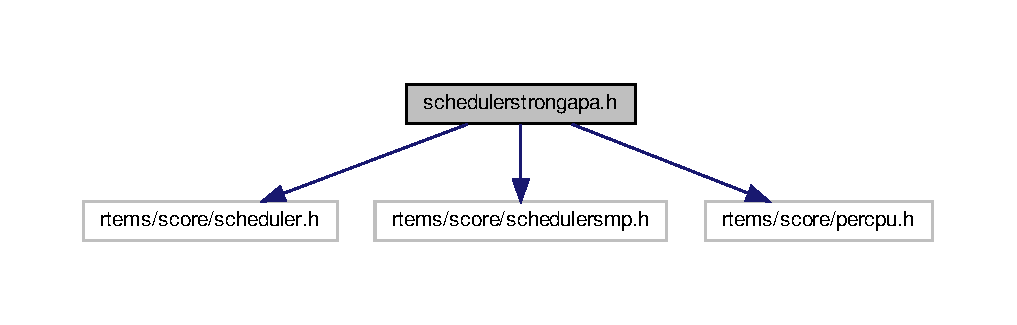
\includegraphics[width=350pt]{schedulerstrongapa_8h__incl}
\end{center}
\end{figure}
\subsection*{Classes}
\begin{DoxyCompactItemize}
\item 
struct \hyperlink{structScheduler__strong__APA__Context}{Scheduler\+\_\+strong\+\_\+\+A\+P\+A\+\_\+\+Context}
\begin{DoxyCompactList}\small\item\em Scheduler context for Strong A\+PA scheduler. \end{DoxyCompactList}\item 
struct \hyperlink{structScheduler__strong__APA__Node}{Scheduler\+\_\+strong\+\_\+\+A\+P\+A\+\_\+\+Node}
\begin{DoxyCompactList}\small\item\em Scheduler node specialization for Strong A\+PA schedulers. \end{DoxyCompactList}\end{DoxyCompactItemize}
\subsection*{Macros}
\begin{DoxyCompactItemize}
\item 
\#define \hyperlink{group__RTEMSScoreSchedulerStrongAPA_ga98b37281082c0be47dc489eed554c5cc}{S\+C\+H\+E\+D\+U\+L\+E\+R\+\_\+\+S\+T\+R\+O\+N\+G\+\_\+\+A\+P\+A\+\_\+\+E\+N\+T\+R\+Y\+\_\+\+P\+O\+I\+N\+TS}
\begin{DoxyCompactList}\small\item\em Entry points for the Strong A\+PA Scheduler. \end{DoxyCompactList}\end{DoxyCompactItemize}
\subsection*{Functions}
\begin{DoxyCompactItemize}
\item 
void \hyperlink{group__RTEMSScoreSchedulerStrongAPA_ga1cde4345d4dc0b5a37a696fa446bb47e}{\+\_\+\+Scheduler\+\_\+strong\+\_\+\+A\+P\+A\+\_\+\+Node\+\_\+initialize} (const Scheduler\+\_\+\+Control $\ast$scheduler, Scheduler\+\_\+\+Node $\ast$node, Thread\+\_\+\+Control $\ast$the\+\_\+thread, Priority\+\_\+\+Control priority)
\begin{DoxyCompactList}\small\item\em Initializes the node with the given priority. \end{DoxyCompactList}\item 
void \hyperlink{group__RTEMSScoreSchedulerStrongAPA_ga0f3ca9f9dcaff88a5df871622caf5e3f}{\+\_\+\+Scheduler\+\_\+strong\+\_\+\+A\+P\+A\+\_\+\+Block} (const Scheduler\+\_\+\+Control $\ast$scheduler, Thread\+\_\+\+Control $\ast$the\+\_\+thread, Scheduler\+\_\+\+Node $\ast$node)
\begin{DoxyCompactList}\small\item\em Blocks the thread. \end{DoxyCompactList}\item 
void \hyperlink{group__RTEMSScoreSchedulerStrongAPA_ga6b96ab0939d82ee5813092159265840e}{\+\_\+\+Scheduler\+\_\+strong\+\_\+\+A\+P\+A\+\_\+\+Unblock} (const Scheduler\+\_\+\+Control $\ast$scheduler, Thread\+\_\+\+Control $\ast$the\+\_\+thread, Scheduler\+\_\+\+Node $\ast$node)
\begin{DoxyCompactList}\small\item\em Unblocks the thread. \end{DoxyCompactList}\item 
void \hyperlink{group__RTEMSScoreSchedulerStrongAPA_ga3cdc0079d2d16a392834bd03b5115ad9}{\+\_\+\+Scheduler\+\_\+strong\+\_\+\+A\+P\+A\+\_\+\+Update\+\_\+priority} (const Scheduler\+\_\+\+Control $\ast$scheduler, Thread\+\_\+\+Control $\ast$the\+\_\+thread, Scheduler\+\_\+\+Node $\ast$node)
\begin{DoxyCompactList}\small\item\em Updates the priority of the node. \end{DoxyCompactList}\item 
bool \hyperlink{group__RTEMSScoreSchedulerStrongAPA_gad863eddc3fa4e2d785fb64af6505e90b}{\+\_\+\+Scheduler\+\_\+strong\+\_\+\+A\+P\+A\+\_\+\+Ask\+\_\+for\+\_\+help} (const Scheduler\+\_\+\+Control $\ast$scheduler, Thread\+\_\+\+Control $\ast$the\+\_\+thread, Scheduler\+\_\+\+Node $\ast$node)
\begin{DoxyCompactList}\small\item\em Asks for help. \end{DoxyCompactList}\item 
void \hyperlink{group__RTEMSScoreSchedulerStrongAPA_ga7809e64065ec5d291f3dc82220a68d3f}{\+\_\+\+Scheduler\+\_\+strong\+\_\+\+A\+P\+A\+\_\+\+Reconsider\+\_\+help\+\_\+request} (const Scheduler\+\_\+\+Control $\ast$scheduler, Thread\+\_\+\+Control $\ast$the\+\_\+thread, Scheduler\+\_\+\+Node $\ast$node)
\begin{DoxyCompactList}\small\item\em Reconsiders help request. \end{DoxyCompactList}\item 
void \hyperlink{group__RTEMSScoreSchedulerStrongAPA_gaf43eb65a6fbbe2826ca4cec68a930cb5}{\+\_\+\+Scheduler\+\_\+strong\+\_\+\+A\+P\+A\+\_\+\+Withdraw\+\_\+node} (const Scheduler\+\_\+\+Control $\ast$scheduler, Thread\+\_\+\+Control $\ast$the\+\_\+thread, Scheduler\+\_\+\+Node $\ast$node, Thread\+\_\+\+Scheduler\+\_\+state next\+\_\+state)
\begin{DoxyCompactList}\small\item\em Withdraws the node. \end{DoxyCompactList}\item 
void \hyperlink{group__RTEMSScoreSchedulerStrongAPA_ga6ac09dac24785561fd7c5ee5bbd8f5ca}{\+\_\+\+Scheduler\+\_\+strong\+\_\+\+A\+P\+A\+\_\+\+Add\+\_\+processor} (const Scheduler\+\_\+\+Control $\ast$scheduler, Thread\+\_\+\+Control $\ast$idle)
\begin{DoxyCompactList}\small\item\em Adds the idle thread to a processor. \end{DoxyCompactList}\item 
Thread\+\_\+\+Control $\ast$ \hyperlink{group__RTEMSScoreSchedulerStrongAPA_gac83f4ab63b404cdfea31e572fa9590a5}{\+\_\+\+Scheduler\+\_\+strong\+\_\+\+A\+P\+A\+\_\+\+Remove\+\_\+processor} (const Scheduler\+\_\+\+Control $\ast$scheduler, struct Per\+\_\+\+C\+P\+U\+\_\+\+Control $\ast$cpu)
\begin{DoxyCompactList}\small\item\em Removes an idle thread from the given cpu. \end{DoxyCompactList}\item 
void \hyperlink{group__RTEMSScoreSchedulerStrongAPA_ga0720c2d79f2b6dd8e91d19879f72b8c7}{\+\_\+\+Scheduler\+\_\+strong\+\_\+\+A\+P\+A\+\_\+\+Yield} (const Scheduler\+\_\+\+Control $\ast$scheduler, Thread\+\_\+\+Control $\ast$the\+\_\+thread, Scheduler\+\_\+\+Node $\ast$node)
\begin{DoxyCompactList}\small\item\em Performs a yield operation. \end{DoxyCompactList}\end{DoxyCompactItemize}
\subsection*{Variables}
\begin{DoxyCompactItemize}
\item 
To Change from \hyperlink{group__RTEMSScoreSchedulerStrongAPA_ga2642e9c7c12fd0dfb1a66f42949a95c4}{here}
\end{DoxyCompactItemize}


\subsection{Detailed Description}
Strong A\+PA Scheduler A\+PI. 


%--- End generated contents ---

% Index
\backmatter
\newpage
\phantomsection
\clearemptydoublepage
\addcontentsline{toc}{chapter}{Index}
\printindex

\end{document}
